\documentclass[12pt, oneside]{article}

\usepackage[letterpaper, scale=0.89, centering]{geometry}
\usepackage{fancyhdr}
\setlength{\parindent}{0em}
\setlength{\parskip}{1em}

\usepackage{tikz}
\usetikzlibrary{automata,positioning,arrows}

\pagestyle{fancy}
\fancyhf{}
\renewcommand{\headrulewidth}{0pt}
\rfoot{\href{https://creativecommons.org/licenses/by-nc-sa/2.0/}{CC BY-NC-SA 2.0} Version \today~(\thepage)}

\usepackage{amssymb,amsmath,pifont,amsfonts,comment,enumerate,enumitem}
\usepackage{currfile,xstring,hyperref,tabularx,graphicx,wasysym}
\usepackage[labelformat=empty]{caption}
\usepackage[dvipsnames,table]{xcolor}
\usepackage{multicol,multirow,array,listings,tabularx,lastpage,textcomp,booktabs}

% NOTE(joe): This environment is credit @pnpo (https://tex.stackexchange.com/a/218450)
\lstnewenvironment{algorithm}[1][] %defines the algorithm listing environment
{   
    \lstset{ %this is the stype
        mathescape=true,
        frame=tB,
        numbers=left, 
        numberstyle=\tiny,
        basicstyle=\rmfamily\scriptsize, 
        keywordstyle=\color{black}\bfseries,
        keywords={,procedure, div, for, to, input, output, return, datatype, function, in, if, else, foreach, while, begin, end, }
        numbers=left,
        xleftmargin=.04\textwidth,
        #1
    }
}
{}
\lstnewenvironment{java}[1][]
{   
    \lstset{
        language=java,
        mathescape=true,
        frame=tB,
        numbers=left, 
        numberstyle=\tiny,
        basicstyle=\ttfamily\scriptsize, 
        keywordstyle=\color{black}\bfseries,
        keywords={, int, double, for, return, if, else, while, }
        numbers=left,
        xleftmargin=.04\textwidth,
        #1
    }
}
{}

\newcommand\abs[1]{\lvert~#1~\rvert}
\newcommand{\st}{\mid}

\newcommand{\A}[0]{\texttt{A}}
\newcommand{\C}[0]{\texttt{C}}
\newcommand{\G}[0]{\texttt{G}}
\newcommand{\U}[0]{\texttt{U}}

\newcommand{\cmark}{\ding{51}}
\newcommand{\xmark}{\ding{55}}


\begin{document}
\begin{flushright}
    \StrBefore{\currfilename}{.}
\end{flushright}

\section*{Before we start}

We are committed to fostering a learning environment for this course that supports a diversity of thoughts, 
perspectives and experiences, and respects your identities (including race, ethnicity, heritage, gender, sex, 
class, sexuality, religion, ability, age, educational background, etc.).  
Our goal is to create a diverse and inclusive learning environment where all students feel comfortable and can thrive. 

If you or someone you know is suffering from food and/or housing insecurities 
there are UCSD resources here to help:

Basic Needs Office: \href{https://basicneeds.ucsd.edu/}{https://basicneeds.ucsd.edu/}

Triton Food Pantry (in the old Student Center)
is free and anonymous, and includes produce: 

\href{https://www.facebook.com/tritonfoodpantry/}{https://www.facebook.com/tritonfoodpantry/}

Mutual Aid UCSD: \href{https://mutualaiducsd.wordpress.com/}{https://mutualaiducsd.wordpress.com/}

Financial aid resources, the possibility of emergency grant funding, and off-campus housing referral 
resources are available. See CAPS and your college dean.

If you find yourself in an uncomfortable situation, ask for help. 
We are committed to upholding University policies regarding nondiscrimination, sexual violence and sexual harassment.

Counseling and Psychological Services (CAPS) at 858 5343755 or \href{http://caps.ucsd.edu}{http://caps.ucsd.edu}


OPHD at (858) 534-8298, ophd@ucsd.edu , \href{http://ophd.ucsd.edu}{http://ophd.ucsd.edu}. 
CARE at Sexual Assault Resource Center at 858 5345793 sarc@ucsd.edu \href{http://care.ucsd.edu}{http://care.ucsd.edu}


Please do not come to class if you are sick or even think you might be sick.
We will continue to follow the campus guidelines as updated on https://returntolearn.ucsd.edu/ .

Please reach out (minnes@ucsd.edu or dgrier@ucsd.edu) if you need support with extenuating circumstances.

\newpage

\section*{Introductions}
Class website: \href{https://canvas.ucsd.edu/courses/45073}{https://canvas.ucsd.edu/courses/45073}


Instructor for A00: Prof. Mia Minnes {\tiny{"Minnes" rhymes with Guinness}}, minnes@ucsd.edu, 
\href{http://cseweb.ucsd.edu/~minnes}{http://cseweb.ucsd.edu/~minnes}

Instructor for B00: Prof. Daniel Grier, dgrier@ucsd.edu, \href{http://danielgrier.com/}{http://danielgrier.com/}

Our team: Two instructors + four TAs and nine tutors + all of you

Fill in contact info for students around you, if you'd like:

\vfill


On a typical week: {\bf MWF} Lectures + review quizzes, {\bf Tu} Homework due, {\bf WF} Discussion.
Office hours (hosted by instructors and TAs and tutors, where you can come to talk 
about course concepts and ask for help as you work through sample problems) and Q+A on Piazza available throughout the week.
All dates are on \href{https://canvas.ucsd.edu/}{Canvas (click for link)} and details are on
 \href{https://canvas.ucsd.edu/courses/45073}{the Syllabus page}.

\newpage Welcome to CSE 105: Introduction to Theory of Computation in Spring 2023!

\section*{CSE 105's Big Questions}
\begin{itemize}
   \item What problems are computers capable of solving?
   \item What resources are needed to solve a problem?
   \item Are some problems harder than others?
\end{itemize}

In this context, a {\bf problem} is defined as: ``Making a decision or computing a value based on some input"

Consider the following problems: 
\begin{itemize}
   \item Find a file on your computer
   \item Determine if your code will compile
   \item Find a run-time error in your code
   \item Certify that your system is un-hackable
\end{itemize}

Which of these is hardest?

\vfill

In Computer Science, we operationalize ``hardest'' as ``requires most resources'', where
resources might be memory, time, parallelism, randomness, power, etc.

To be able to compare ``hardness'' of problems, we use a consistent description of problems

{\bf Input}: String

{\bf Output}: Yes/ No, where Yes means that the input string matches the pattern or property described by the problem.


\newpage
\section*{Monday}

%! app: Regular Languages
%! outcome: Define decision problem

We will use vocabulary that should be familiar from your discrete 
math and introduction to proofs classes.  Some of the notation conventions may 
be a bit different: we will use the notation from this class' textbook\footnote{Page references are to 
the 3rd edition (International) of Siper's Introduction to the Theory of Computation,
available at the campus bookstore for under \$20. Copies of the book are also available 
for those who can't access the book
to borrow from the course instructor, while supplies last (minnes@eng.ucsd.edu)}.

Write out in words the meaning of the symbols below: 
\[
    \{ a,b, c\}
\]

\phantom{The set whose elements are $a$, $b$, and $c$}

\[
    | \{a, b, a \} | = 2
\]

\phantom{The number of elements in the set $\{a,b,a\}$ is $2$.}

\[
    | aba | = 3
\]

\phantom{The length of the string $aba$ is $3$.}

\[
    (a, 3, 2, b, b)
\]

\phantom{The $5$-tuple whose first components is $a$, second component 
is $3$, third component is $2$, fourth component is $b$, and fifth component is $b$.}



\begin{center}
    \begin{tabular}{|p{2in}cp{4in}|}
    \hline 
    Term & Typical symbol & Meaning \\
    \hline\hline
    Alphabet & $\Sigma$, $\Gamma$ & A non-empty finite set	 \\ \hline
    Symbol over $\Sigma$  & $\sigma$, $b$, $x$ & An element of the alphabet $\Sigma$\\ \hline
    String over $\Sigma$  &	$u$, $v$, $w$ & A finite list of symbols from $\Sigma$\\ \hline
    The set of all strings over $\Sigma$ & $\Sigma^*$ & The collection of all possible strings formed from symbols from $\Sigma$ \\ \hline
    (Some) language over $\Sigma$& $L$ & (Some) set of strings over $\Sigma$ \\ \hline
    Empty string &$\varepsilon$ & The string of length $0$\\ \hline
    Empty set &$\emptyset$ & The empty language\\ \hline
    Natural numbers &$\mathcal{N}$ & The set of positive integers \\ \hline
    Finite set & & The empty set or a set whose distinct elements can be counted by a natural number\\ \hline
    Infinite set & & A set that is not finite.\\ 
    \hline\hline
    {\it Pages 3, 4, 13, 14 }& & \\
    \hline
    \end{tabular}
\end{center}

\newpage

\begin{center}
    \begin{tabular}{|p{2.7in}cp{3.8in}|}
    \hline
    Term & Notation & Meaning \\
    \hline \hline
    Reverse of a string $w$ & $w^\mathcal{R}$  & write $w$  in  the opposite order, if $w = w_1 \cdots  w_n$ then $w^\mathcal{R} = w_n \cdots  w_1$. Note: $\varepsilon^\mathcal{R} = \varepsilon$\\ \hline
    Concatenating strings $x$ and $y$ & $xy$ &  take $x = x_1 \cdots x_m$, $y=y_1 \cdots y_n$ and form $xy = x_1 \cdots x_m y_1 \cdots y_n$\\ \hline
    String $z$ is a substring of string $w$ & & there are strings $u,v$ such that $w = uzv$\\ \hline
    String $x$ is a prefix of string $y$ & & there is a string $z$ such that $y = xz$ \\ \hline
    String $x$ is a proper prefix of string $y$ & & $x$ is a prefix of $y$ and $x \neq y$\\ \hline
    Shortlex order, also known as string order over alphabet $\Sigma$ & & Order strings over  $\Sigma$ first by length and then according to the dictionary order, assuming symbols in $\Sigma$  have an ordering.\\ \hline
    \hline \hline
    {\it Pages 13, 14} & & \\
    \hline
    \end{tabular}
\end{center}

    

{\it Circle the correct choice}:

A {\bf string} over an alphabet $\Sigma$ is \underline{~~an element of $\Sigma^*$ ~~ OR ~~ a subset of $\Sigma^*$}.
    
A {\bf language} over an alphabet $\Sigma$ is \underline{~~an element of $\Sigma^*$ ~~ OR ~~ a subset of $\Sigma^*$}.


{\it Extra examples for practice:}

With $\Sigma_1 = \{0,1\}$ and $\Sigma_2 = \{a,b,c,d,e,f,g,h,i,j,k,l,m,n,o,p,q,r,s,t,u,v,w,x,y,z\}$  and $\Gamma = \{0,1,x,y,z\}$

An example of a string of length 3 over $\Sigma_1$ is \underline{\phantom{ $000$} \hspace{0.2in}}

An example of  a string of length 1 over $\Sigma_2$ is  \underline{\phantom{ $k$} \hspace{0.2in}}

The number of distinct strings of length 2 over $\Gamma$ is  \underline{\phantom{ $25$} \hspace{0.2in}}

An example of a language over $\Sigma_1$ of size $1$ is  \underline{\phantom{ $ \{ \varepsilon \} $} \hspace{0.2in}}

An example of an infinite language over $\Sigma_1$ is  \underline{\phantom{ $\Sigma^*$} \hspace{0.2in}}
    
An example of  a finite language over $\Gamma$ is  \underline{\phantom{ $\{ 0, x \}$} \hspace{0.2in}}
    
{\bf True} or {\bf False}: $\varepsilon \in \Sigma_1$

{\bf True} or {\bf False}: $\varepsilon$ is  a string over $\Sigma_1$

{\bf True} or {\bf False}: $\varepsilon$ is a language over $\Sigma_1$

{\bf True} or {\bf False}: $\varepsilon$ is a prefix of some string over  $\Sigma_1$

{\bf True} or {\bf False}: There is a string over $\Sigma_1$ that is a proper prefix of $\varepsilon$
    

The first five strings over $\Sigma_1$ in string order, using the ordering $0 <  1$: \vfill
    
The first five strings over $\Sigma_2$ in string order, using the usual alphabetical ordering for single letters: \vfill

    
\newpage
\subsection*{Review: Week 1 Monday}
\begin{enumerate}
\item Please complete the beginning of the quarter survey linked from our \#FinAid
Assignment on Canvas \href{https://canvas.ucsd.edu/courses/45073/assignments/609253}{https://canvas.ucsd.edu/courses/45073/assignments/609253?wrap=1}
\item We want you to be familiar with class policies and procedures so you are ready to have a successful quarter. 
Please take a look at the syllabus on our class website https://canvas.ucsd.edu/courses/45073
and answer the questions about it on Gradescope.
\end{enumerate}

A summary of the terminology we will use is on page 16 in the textbook.

{\bf Pre class reading for next time}: Example 1.51, Definition 1.52

{\it Notice}: we are jumping to Section 1.3 Regular Expressions and then will come back 
to Section 1.1 Finite Automata on Friday.


\newpage
\subsection*{Week 1 Wednesday}

%! app: Regular Languages
%! outcome: Regular expressions

Our motivation in studying sets of strings is that they can be used to encode problems.
To calibrate how difficult a problem is to solve, we describe how complicated the set of strings that encodes it is. 
How do we define sets of strings?


\vfill

How would you describe the language that has no elements at all?

\vfill

How would you describe the language that has all strings over $\{0,1\}$ as its elements?

\vfill

\newpage


{\bf Definition 1.52}: A {\bf regular expression} over alphabet $\Sigma$
is a syntactic expression that can describe a language over $\Sigma$. The collection of all regular
expressions is defined recursively:
\begin{itemize}
\item[] {\it Basis steps of recursive definition}
\begin{quote}    
    $a$ is a regular expression, for $a \in \Sigma$

    $\varepsilon$ is a regular expression

    $\emptyset$ is a regular expression
\end{quote}

\item[] {\it Recursive steps of recursive definition}
\begin{quote}
    $(R_1 \cup R_2)$ is a regular expression when $R_1$, $R_2$ are regular expressions 

    $(R_1 \circ R_2)$ is a regular expression when $R_1$, $R_2$ are regular expressions

    $(R_1^*)$ is a regular expression when $R_1$ is a regular expression 
\end{quote}
\end{itemize}
 

The {\it semantics} (or meaning) of the syntactic regular expression is the {\bf language
described by the regular expression}. The function that assigns a language to a regular expression
over $\Sigma$ is defined recursively, using familiar set operations:


\begin{itemize}
    \item[] {\it Basis steps of recursive definition}
    \begin{quote}    
        The language described by $a$, for $a \in \Sigma$, is $\{a\}$ and we write 
        $L(a) = \{a\}$
    
        The language described by $\varepsilon$ is $\{\varepsilon\}$ and we write 
        $L(\varepsilon) = \{ \varepsilon\}$
    
        The language described by $\emptyset$ is $\{\}$ and we write
        $L(\emptyset) = \emptyset$.
    \end{quote}
    
    \item[] {\it Recursive steps of recursive definition}
    \begin{quote}
        When $R_1$, $R_2$ are regular expressions, the language described by the regular
        expression $(R_1 \cup R_2)$ is the union of the languages described by $R_1$ and $R_2$, 
        and we write 
        $$L(~(R_1 \cup R_2)~) = L(R_1) \cup L(R_2) = \{ w \mid w \in L(R_1) \lor w \in L(R_2)\}$$
    
        When $R_1$, $R_2$ are regular expressions, the language described by the regular
        expression $(R_1 \circ R_2)$ is the concatenation of the languages described by $R_1$ and $R_2$, 
        and we write 
        $$L(~(R_1 \circ R_2)~) = L(R_1) \circ L(R_2) = \{ uv \mid u \in L(R_1) \land v \in L(R_2)\}$$
    
        When $R_1$ is a regular expression, the language described by the regular 
        expression $(R_1^*)$ is the {\bf Kleene star} of the language described by $R_1$ and we write
        $$L(~(R_1^*)~) = (~L(R_1)~)^* = \{ w_1 \cdots w_k \mid k \geq 0 \textrm{ and each } w_i \in L(R_1)\}$$
    \end{quote}
\end{itemize}
  
For the following examples assume the alphabet is $\Sigma_1 =  \{0,1\}$:
    
The language described by the regular expression $0$ is $L(0) = \{ 0 \}$

The language described by the regular expression $1$ is $L(1)  = \{ 1 \}$

The language described by the regular expression $\varepsilon$ is $L(\varepsilon) = \{ \varepsilon  \}$

The language described by the regular expression $\emptyset$ is $L(\emptyset) = \emptyset$

The language described by the regular expression $((0 \cup 1) \cup 1)$ is $L(~((0 \cup 1) \cup 1)~) = $

\vfill

The language described by the regular expression $1^+$ is $L(~(1)^+~) = $

\vfill

The language described by the regular expression $\Sigma_1^* 1$ is $L(~\Sigma_1^* 1~) = $

\vfill

The language described by the regular expression $(\Sigma_1 \Sigma_1 \Sigma_1 \Sigma_1 \Sigma_1)^*$ 
is $L(~(\Sigma_1 \Sigma_1 \Sigma_1 \Sigma_1 \Sigma_1)^*~) = $

\vfill

A regular expression that describes the language $\{00, 01, 10, 11\}$ is 

\vfill

A regular expression that describes the language $\{ 0^n1 \mid n~\text{is even} \}$ is

\vfill

{\it Shorthand and conventions}
    
\begin{center}
    \begin{tabular}{|ll|}
    \hline
    \multicolumn{2}{|l|}{Assuming $\Sigma$ is the alphabet, we use the following conventions}\\
    \hline
    $\Sigma$   & regular  expression describing language consisting of  all strings  of length  $1$ over $\Sigma$\\
    $*$ then $\circ$ then $\cup$   & precedence order, unless parentheses are used to change it\\
    $R_1R_2$ & shorthand  for  $R_1  \circ R_2$ (concatenation symbol is implicit) \\
    $R^+$ & shorthand for $R^* \circ R$ \\
    $R^k$ & shorthand for $R$ concatenated with itself $k$ times, where $k$ is a natural number\\
    \hline
    {\it Pages 63 - 65 }& \\
    \hline
    \end{tabular}
\end{center}

\newpage
{\bf Caution: many programming languages that support regular expressions build in functionality
that is more powerful than the ``pure'' definition of regular expressions given here. }

Regular expressions are everywhere (once you start looking for them).

Software tools and languages often have built-in support for regular expressions to describe
{\bf patterns} that we want to match (e.g. Excel/ Sheets, grep, Perl, python, Java, Ruby).

Under the hood, the first phase of {\bf compilers} is to transform the strings we write 
in code to tokens (keywords, operators, identifiers, literals). Compilers use regular expressions
to describe the sets of strings that can be used for each token type.

Next time: we'll start to see how to build machines that decide whether strings match the pattern
described by a regular expression.

\vfill


{\it Extra examples for practice:}

Which regular expression(s) below describe a language that includes the string $a$ as an element?

$a^* b^*$ 

\vfill

$a(ba)^* b$

\vfill

$a^* \cup b^*$

\vfill

$(aaa)^*$

\vfill

$(\varepsilon \cup a) b$

\vfill

\newpage
\subsection*{Review: Week 1 Wednesday}

Please complete the review quiz questions on \href{http://gradescope.com}{Gradescope} about 
strings, languages, and regular expressions.


Recall: Review quizzes based on class material are assigned each day. 
These quizzes will help you track and confirm your understanding of the concepts and examples 
we work in class. Quizzes can be submitted on Gradescope as many times (with no penalty) as 
you like until the quiz deadline: the three quizzes each week are all due on Friday (with no penalty 
late submission open until Sunday).

The definition of the union, concatenation, and star operations for languages is given 
as Definition 1.23 on page 44 and a useful example is Example 1.24.

{\bf Pre class reading for next time}: Figure 1.4, Definition 1.5

{\it Notice}: On Friday we are going back to the start of Chapter 1 and will be discussing finite 
automata and their computations.

\newpage
\subsection*{Week 1 Friday}

%! app: regular-languages, 
%! outcome: Regular expressions, Formal definition of automata, Informal definition of automata

{\bf Review}: Determine whether each statement below about regular expressions
over the alphabet $\{a,b,c\}$ is true or false:
   
True or False: \qquad 
   $a  \in L(~(a \cup b )~\cup c)$

True or False: \qquad 
   $ab  \in L(~ (a \cup b)^*  ~)$
   
True or False: \qquad    
   $ba \in L( ~ a^* b^* ~)$
   
True or False: \qquad 
   $\varepsilon  \in L(a \cup b \cup c)$
   
True or False: \qquad 
   $\varepsilon  \in L(~ (a \cup b)^*  ~)$

True or False: \qquad 
   $\varepsilon \in L( ~ a^* b^* ~)$


{\bf From the pre-class reading, pages 34-36}:
A deterministic finite automaton (DFA) is specified by  $M = (Q, \Sigma, \delta, q_0, F)$.
This $5$-tuple is called the {\bf formal definition} of the DFA. The DFA can also 
be represented by its state diagram: with nodes for the state, labelled edges specifying the 
transition function, and decorations on nodes denoting the start and accept states.

\begin{quote}
Finite set of states $Q$ can be labelled by any collection of distinct names. Often
we use default state labels $q0, q1, \ldots$ 
\end{quote}

\begin{quote}  
The alphabet $\Sigma$ determines the possible inputs to the automaton. 
Each input to the automaton is a string over  $\Sigma$, and the automaton ``processes'' the input
one symbol (or character) at a time.
\end{quote}

\begin{quote}
The transition function $\delta$ gives the next state of the DFA based on the current state of 
the machine and on the next input symbol.
\end{quote}

\begin{quote}
The start state $q_0$ is an element of $Q$.  Each computation of the machine starts at the  start  state.
\end{quote}

\begin{quote}
The accept (final) states $F$ form a subset of the states of the DFA, $F \subseteq  Q$. 
These states are used to flag if the machine accepts or rejects an input string.
\end{quote}


\begin{quote}
The computation of a machine on an input string is a sequence of states
in the machine,  starting with the start state, determined by transitions 
of the machine as it reads successive input symbols.
\end{quote}

\begin{quote}
The DFA $M$ accepts the given input string exactly when the computation of $M$ on the input string
ends in an accept state. $M$ rejects the given input string exactly when the computation of 
$M$ on the input string ends in a nonaccept state, that is, a state that is not in $F$.
\end{quote}

\begin{quote} 
The language of $M$, $L(M)$, is defined as the set of  all strings that are each accepted 
by the machine $M$. Each string that is rejected by $M$ is not in $L(M)$.
The language of $M$ is also called the language recognized by $M$.
\end{quote}   
   
What is {\bf finite} about all deterministic finite automata? (Select all that apply)
\begin{itemize}
   \item[$\square$] The size of the machine (number of states, number of arrows)
   \item[$\square$] The number of strings that are accepted by the machine
   \item[$\square$] The length of each computation of the machine
\end{itemize}
  
\begin{figure}[h]
   \centering
   \includegraphics[width=3in]{../../resources/machines/Lect2DFA1.png} 
\end{figure}
   
The formal definition of this DFA is
   
\vspace{100pt}
   

Classify each string $a, aa, ab, ba, bb, \varepsilon$ as accepted by the DFA or rejected by the DFA.  

{\it Why are these the only two options?}

\vspace{200pt}


The language recognized by this DFA is
  
\vspace{100pt}
   

\begin{figure}[h]
  \centering
  \includegraphics[width=3in]{../../resources/machines/Lect2DFA2.png} 
\end{figure}
   

The language recognized by this DFA is
  
\vspace{100pt}

\begin{figure}[h]
    \centering
    \includegraphics[width=3in]{../../resources/machines/Lect2DFA3.png} 
\end{figure}

The language recognized by this DFA is
  
\vspace{100pt}



\newpage

\subsection*{Review: Week 1 Friday}

Please complete the review quiz questions on \href{http://gradescope.com}{Gradescope} about 
DFA and the strings they accept and reject.

The definition of the union, concatenation, and star operations for languages is given 
as Definition 1.23 on page 44 and a useful example is Example 1.24.


The first homework assignment for CSE 105 this quarter is due next week. 
Find it on the class website: in the Calendar section of the website, click on the link under "Due Dates" for Week 2, or find
the detailed assignment in the Assignments section of the website.
Due: 4/11/23 at 5pm (no penalty late submission until 8am next morning)

We encourage you to work on homework in groups of up to three CSE 105 classmates. 
To find group members: reach out to people sitting around you in class, in discussion section, 
or during office hours. The pre-survey also asks if you want help finding group members: 
the CSE 105 instructional team can help you connect with other students. Working within the 
campus safety guidelines, you may choose to meet with your group mates in person or remotely. 
We highly recommend meeting synchronously so that you can work through the homework problems *together*. 

{\bf Pre class reading for next time}: pages 41-43 (figures 1.18, 1.19, 1.20)

\newpage

{\it Textbook references: Within a chapter, each item is numbered consecutively. Figure 1.22
is the twenty-second numbered item in chapter one; it comes right after Example 1.21 and right before Definition 1.23.}

In Computer Science, we operationalize ``hardest'' as ``requires most resources'', where
resources might be memory, time, parallelism, randomness, power, etc.
To be able to compare ``hardness'' of problems, we use a consistent description of problems

{\bf Input}: String

{\bf Output}: Yes/ No, where Yes means that the input string matches the pattern or property described by the problem.

So far: we saw that regular expressions are convenient ways of describring patterns in strings.
DFA give a model of computation for processing strings and and classifying them into Yes (accepted)
or No (rejected). We will see that each set of strings is described by a regular expression if and only 
if there is a DFA that recognizes it.  Another way of thinking about it: properties described by regular
expressions require exactly the computational power of DFAs.


\section*{Monday}

%! app: Regular Languages
%! outcome: Regular expressions, Formal definition of automata, Informal definition of automata


{\bf Review}: Formal definition of DFA: $M = (Q, \Sigma, \delta, q_0, F)$ 

\begin{center}
\begin{multicols}{2}
\begin{itemize}
\setlength{\itemsep}{2pt}
\item Finite set of states $Q$
\item Alphabet $\Sigma$
\item Transition function $\delta$
\item Start state $q_0$
\item Accept (final) states $F$
\end{itemize}
\end{multicols}
\end{center}
In the state diagram of $M$, how many outgoing arrows are there from each state?

$M = ( \{ q, r, s\}, \{a,b\}, \delta, q, \{s\} )$ 
where $\delta$ is  (rows labelled by states
and columns labelled by symbols):
\begin{center}
\begin{tabular}{c|cc}
$\delta$ & $a$ & $b$ \\
\hline
$q$ & $r$ & $q$ \\
$r$ & $r$ & $s$ \\
$s$ & $s$ & $s$ \\
\end{tabular}
\end{center}

The state diagram for $M$ is 

\vfill



Give two examples of strings that are accepted by $M$ and two examples of strings that are rejected by $M$:

\vfill

Add ``labels" for states in the state diagram, e.g. ``have not seen any of desired pattern yet'' or
``sink state''.
\newpage

We can use the analysis of the roles of the states in the state diagram to describe the language
recognized by the DFA. 


$L(M) = $

A regular expression describing $L(M)$ is




\vspace{300pt}

Let the alphabet be $\Sigma_1 = \{0,1\}$.

A state diagram for a DFA that recognizes $\{w \mid w~\text{contains at most two $1$'s} \}$ is

\vspace{70pt}

A state diagram for a DFA that recognizes $\{w \mid w~\text{contains more than two $1$'s} \}$ is

\vspace{70pt}


\newpage
{\it Extra example:} A state diagram for DFA recognizing
$$\{w \mid w~\text{is a string over $\{0,1\}$ whose length is not a multiple of $3$} \}$$

\vspace{70pt}


Let $n$ be an arbitrary positive integer. What is a formal definition for a DFA recognizing
\[
\{w \mid w~\text{is a string over $\{0,1\}$ whose length is not a multiple of $n$} \}?
\]

\vspace{70pt}
    
\newpage
\subsection*{Review: Week 2 Monday}

Please complete the review quiz questions on \href{http://gradescope.com}{Gradescope} about 
the languages recognized by DFAs.


Recall: Review quizzes based on class material are assigned each day. 
These quizzes will help you track and confirm your understanding of the concepts and examples 
we work in class. Quizzes can be submitted on Gradescope as many times (with no penalty) as 
you like until the quiz deadline: the three quizzes each week are all due on Friday (with no penalty 
late submission open until Sunday).

{\bf Pre class reading for next time}: Pages 45-47.


\newpage
\subsection*{Wednesday}

%! app: Regular Languages
%! outcome: Regular expressions, Formal definition of automata, Informal definition of automata

Suppose A is a language over an alphabet $\Sigma$. By definition, this means A is a subset of $\Sigma^*$.
{\bf Claim:} if there is a DFA $M$ such that $L(M) = A$ then there is another DFA, let's call it $M'$, such that 
$L(M') = \overline{A}$, the complement of $A$, defined as $\{ w \in \Sigma^* \mid w \notin A \}$.

{\bf Proof idea}:


{\bf Proof}: 




\vfill
A useful (optional) bit of terminology: the {\bf iterated transition function} of a DFA
$M = (Q, \Sigma, \delta, q_0, F)$ is defined recursively by
\[
\delta^* (~(q,w)~) 
=\begin{cases}
q  \qquad &\text{if $q \in Q, w = \varepsilon$} \\
\delta( ~(q,a)~) \qquad &\text{if $q \in Q$, $w = a \in \Sigma$ } \\
\delta(~(\delta^*(q,u), a) ~) \qquad &\text{if $q \in Q$, $w = ua$ where $u \in  \Sigma^*$ and $a \in \Sigma$}
\end{cases}
\]

Using  this terminology, $M$ accepts a string $w$ over $\Sigma$ if and only if $\delta^*( ~(q_0,w)~) \in F$.

\newpage

Fix  $\Sigma = \{a,b\}$. A state diagram for a DFA that recognizes 
$\{w \mid w~\text{has $ab$ as a substring and is of even length} \}$:


\vspace{120pt}


Suppose $A_1, A_2$ are languages over an alphabet $\Sigma$.
{\bf Claim:} if there is a DFA $M_1$ such that $L(M_1) = A_1$ and 
DFA $M_2$ such that $L(M_2) = A_2$, then there is another DFA, let's call it $M$, such that 
$L(M) = A_1 \cap A_2$.

{\bf Proof idea}:


{\bf Formal construction}: 


\vspace{70pt}

{\bf Application}:  When $A_1 = \{w \mid w~\text{has $ab$ as a substring} \}$ and 
$A_2 = \{ w \mid w~\text{is of even length} \}$.


\newpage

Suppose $A_1, A_2$ are languages over an alphabet $\Sigma$.
{\bf Claim:} if there is a DFA $M_1$ such that $L(M_1) = A_1$ and 
DFA $M_2$ such that $L(M_2) = A_2$, then there is another DFA, let's call it $M$, such that 
$L(M) = A_1 \cup A_2$.  {\it Sipser Theorem 1.25, page 45}

{\bf Proof idea}:


{\bf Formal construction}: 

\vspace{70pt}

{\bf Application}: A state diagram for a DFA that recognizes $\{w \mid w~\text{has $ab$ as a substring or is of even length} \}$:

\vspace{100pt}


\newpage
\subsection*{Review: Week 2 Wednesday}

Please complete the review quiz questions on \href{http://gradescope.com}{Gradescope} about 
the languages recognized by DFAs.


Recall: Review quizzes based on class material are assigned each day. 
These quizzes will help you track and confirm your understanding of the concepts and examples 
we work in class. Quizzes can be submitted on Gradescope as many times (with no penalty) as 
you like until the quiz deadline: the three quizzes each week are all due on Friday (with no penalty 
late submission open until Sunday).


{\bf Pre class reading for next time}: Introduction to Section 1.2

\newpage
\subsection*{Friday}

%! app: Regular Languages
%! outcome: Formal definition of automata, Informal definition of automata, Nondeterminism


\begin{center}
\begin{tabular}{|ll|}
\hline
\multicolumn{2}{|l|}{{\bf Nondeterministic finite automaton} $M = (Q, \Sigma, \delta, q_0, F)$} \\
Finite set of states $Q$  & Can  be labelled by any collection  of distinct names. Default: $q0, q1, \ldots$  \\
Alphabet $\Sigma$ &  Each input to the automaton is a string over  $\Sigma$. \\
Arrow labels $\Sigma_\varepsilon$ &  $\Sigma_\varepsilon = \Sigma \cup \{ \varepsilon\}$. \\
&  Arrows 
in the state diagram are labelled either by symbols from $\Sigma$ or by $\varepsilon$ \\
Transition function $\delta$  & $\delta: Q \times \Sigma_{\varepsilon} \to \mathcal{P}(Q)$
gives the {\bf set of possible next states} for a transition \\
&  from the current state upon reading a symbol or spontaneously moving.\\
Start state $q_0$ & Element of $Q$.  Each computation of the machine starts at the  start  state.\\
Accept (final) states $F$ & $F \subseteq  Q$.\\
$M$ accepts the input string & if and only if {\bf there is} a computation of $M$ on the input string\\
&  that 
processes the whole string and ends in an
accept state.\\
\hline
{\it Page 53}& \\
\hline
\end{tabular}
\end{center}

The formal definition of the NFA over $\{0,1\}$ given by this state diagram is: 

\includegraphics[width=2in]{../../resources/machines/Lect4NFA1.png}

The language over $\{0,1\}$ recognized by this NFA is:

\vspace{70pt}

Change the transition function to get a different NFA which accepts
the empty string.


\newpage

The state diagram of an NFA over $\{a,b\}$ is below.  The formal definition of this NFA is:

\vspace{-30pt}

\includegraphics[width=2.5in]{../../resources/machines/Lect5NFA1.png}


\vspace{-10pt}

The language recognized by this NFA is: 


\newpage

\subsection*{Review: Week 2 Friday}


Please complete the review quiz questions on \href{http://gradescope.com}{Gradescope} about 
NFA.

{\bf Pre class reading for next time}: Theorem 1.47, Theorem 1.49

\newpage

\section*{Monday}

%! app: regular-languages
%! outcome: Formal definition of automata, Informal definition of automata, Nondeterminism

The state diagram of an NFA over $\{a,b\}$ is below.  The formal definition of this NFA is:

\includegraphics[width=2.5in]{../../resources/machines/Lect5NFA1.png}

The language recognized by this NFA is: 



Suppose $A_1, A_2$ are languages over an alphabet $\Sigma$.
{\bf Claim:} if there is a NFA $N_1$ such that $L(N_1) = A_1$ and 
NFA $N_2$ such that $L(N_2) = A_2$, then there is another NFA, let's call it $N$, such that 
$L(N) = A_1 \cup A_2$.

{\bf Proof idea}: Use nondeterminism to choose which of $N_1$, $N_2$ to run.


{\bf Formal construction}: Let 
$N_1 = (Q_1, \Sigma, \delta_1, q_1, F_1)$ and $N_2 = (Q_2, \Sigma, \delta_2,q_2, F_2)$
and assume $Q_1 \cap Q_2 = \emptyset$ and that $q_0 \notin Q_1 \cup Q_2$.
Construct $N = (Q, \Sigma, \delta, q_0, F_1 \cup F_2)$ where
\begin{itemize}
    \item $Q = $
    \item $\delta: Q \times \Sigma_\varepsilon \to \mathcal{P}(Q)$ is defined by, for $q \in Q$ and $a \in \Sigma_{\varepsilon}$:
        \[
            \phantom{\delta((q,a))=\begin{cases}  \delta_1 ((q,a)) &\qquad\text{if } q\in Q_1 \\ \delta_2 ((q,a)) &\qquad\text{if } q\in Q_2 \\ \{q1,q2\} &\qquad\text{if } q = q_0, a = \varepsilon \\ \emptyset\text{if } q= q_0, a \neq \varepsilon \end{cases}}
        \]
\end{itemize}


\vfill
{\it Proof of correctness would prove that $L(N) = A_1 \cup A_2$ by considering
an arbitrary string accepted by $N$, tracing an accepting computation of $N$ on it, and using 
that trace to prove the string is in at least one of $A_1$, $A_2$; then, taking an arbitrary 
string in $A_1 \cup A_2$ and proving that it is accepted by $N$. Details left for extra practice.}

\newpage
Over the alphabet $\{a,b\}$, the language $L$ described by the regular expression 
$\Sigma^* a \Sigma^* b$

 includes the strings \phantom{space for strings here} and excludes the strings 


The state diagram of a NFA recognizing $L$ is:

\vspace{100pt}

Suppose $A_1, A_2$ are languages over an alphabet $\Sigma$.
{\bf Claim:} if there is a NFA $N_1$ such that $L(N_1) = A_1$ and 
NFA $N_2$ such that $L(N_2) = A_2$, then there is another NFA, let's call it $N$, such that 
$L(N) = A_1 \circ A_2$.

{\bf Proof idea}: Allow computation to move between $N_1$ and $N_2$ ``spontaneously" when reach an accepting state of 
$N_1$, guessing that we've reached the point where the two parts of the string in the set-wise concatenation 
are glued together.


{\bf Formal construction}: Let 
$N_1 = (Q_1, \Sigma, \delta_1, q_1, F_1)$ and $N_2 = (Q_2, \Sigma, \delta_2,q_2, F_2)$
and assume $Q_1 \cap Q_2 = \emptyset$.
Construct $N = (Q, \Sigma, \delta, q_0, F)$ where
\begin{itemize}
    \item $Q = $
    \item $q_0 = $
    \item $F = $
    \item $\delta: Q \times \Sigma_\varepsilon \to \mathcal{P}(Q)$ is defined by, for $q \in Q$ and $a \in \Sigma_{\varepsilon}$:
        \[
            \delta((q,a))=\begin{cases}  
                \delta_1 ((q,a)) &\qquad\text{if } q\in Q_1 \textrm{ and } q \notin F_1\\ 
                \delta_1 ((q,a)) &\qquad\text{if } q\in F_1 \textrm{ and } a \in \Sigma\\ 
                \delta_1 ((q,a)) \cup \{q_2\} &\qquad\text{if } q\in F_1 \textrm{ and } a = \varepsilon\\ 
                \delta_2 ((q,a)) &\qquad\text{if } q\in Q_2
            \end{cases}
        \]
\end{itemize}

\vfill

{\it Proof of correctness would prove that $L(N) = A_1 \circ A_2$ by considering
an arbitrary string accepted by $N$, tracing an accepting computation of $N$ on it, and using 
that trace to prove the string can be written as the result of concatenating two strings, 
the first in $A_1$ and the second in $A_2$; then, taking an arbitrary 
string in $A_1 \circ A_2$ and proving that it is accepted by $N$. Details left for extra practice.}

\newpage

Suppose $A$ is a language over an alphabet $\Sigma$.
{\bf Claim:} if there is a NFA $N$ such that $L(N) = A$, then there is another NFA, let's call it $N'$, such that 
$L(N') = A^*$.

{\bf Proof idea}: Add a fresh start state, which is an accept state. Add spontaneous 
moves from each (old) accept state to the old start state.

{\bf Formal construction}: Let 
$N = (Q, \Sigma, \delta, q_1, F)$ and assume $q_0 \notin Q$.
Construct $N' = (Q', \Sigma, \delta', q_0, F')$ where
\begin{itemize}
    \item $Q' = Q \cup \{q_0\}$
    \item $F' = F \cup \{q_0\}$
    \item $\delta': Q' \times \Sigma_\varepsilon \to \mathcal{P}(Q')$ is defined by, for $q \in Q'$ and $a \in \Sigma_{\varepsilon}$:
        \[
            \delta'((q,a))=\begin{cases}  
                \delta ((q,a)) &\qquad\text{if } q\in Q \textrm{ and } q \notin F\\ 
                \delta ((q,a)) &\qquad\text{if } q\in F \textrm{ and } a \in \Sigma\\ 
                \delta ((q,a)) \cup \{q_1\} &\qquad\text{if } q\in F \textrm{ and } a = \varepsilon\\ 
                \{q_1\} &\qquad\text{if } q = q_0 \textrm{ and } a = \varepsilon \\
                \emptyset &\qquad\text{if } q = q_0 \textrm { and } a \in \Sigma
            \end{cases}
        \]
\end{itemize}


{\it Proof of correctness would prove that $L(N') = A^*$ by considering
an arbitrary string accepted by $N'$, tracing an accepting computation of $N'$ on it, and using 
that trace to prove the string can be written as the result of concatenating some number of strings, 
each of which is in $A$; then, taking an arbitrary 
string in $A^*$ and proving that it is accepted by $N'$. Details left for extra practice.}


{\bf Application}: A state diagram for a NFA over $\Sigma = \{a,b\}$ 
that recognizes $L (( \Sigma^* b)^* )$:

\vspace{200pt}




{\bf True} or {\bf False}: The state diagram of any DFA is also the state diagram of a NFA.

{\bf True} or {\bf False}: The state diagram of any NFA is also the state diagram of a DFA.

{\bf True} or {\bf False}: The formal definition $(Q, \Sigma, \delta, q_0, F)$ of any DFA is also the formal definition of a NFA.

{\bf True} or {\bf False}: The formal definition $(Q, \Sigma, \delta, q_0, F)$  of any NFA is also the formal definition of a DFA.


    
\subsection*{Review: Week 3 Monday}


Recall: Review quizzes based on class material are assigned each day. 
These quizzes will help you track and confirm your understanding of the concepts and examples 
we work in class. Quizzes can be submitted on Gradescope as many times (with no penalty) as 
you like until the quiz deadline: the three quizzes each week are all due on Friday (with no penalty 
late submission open until Sunday).

Please complete the review quiz questions on \href{http://gradescope.com}{Gradescope} about 
constructions using NFAs.

{\bf Pre class reading for next time}: Theorem 1.39 ``Proof Idea'', Example 1.41, Example 1.56, Example 1.58.


\newpage
\subsection*{Wednesday}

%! app: regular-languages
%! outcome: Regular expressions, Formal definition of automata, Informal definition of automata, Nondeterminism


Consider the state diagram of an NFA over $\{a,b\}$:

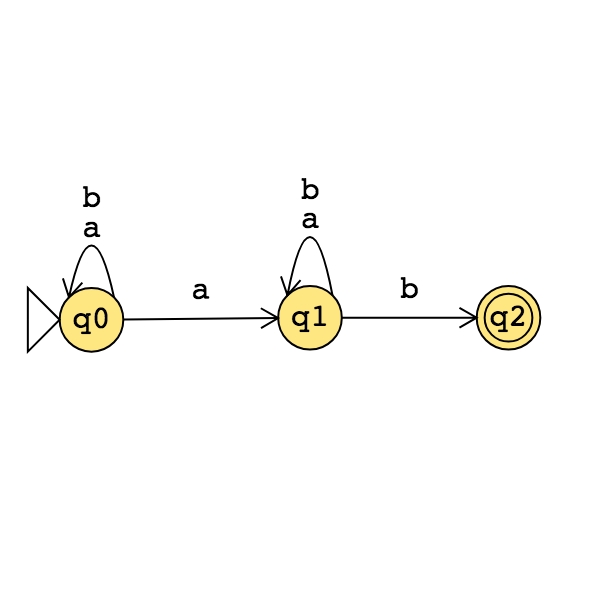
\includegraphics[width=2.5in]{../../resources/machines/Lect6NFA1.png}


The language recognized by this NFA is



The state diagram of a DFA recognizing this same language is:

\vspace{70pt}
Suppose $A$ is a language over an alphabet $\Sigma$.
{\bf Claim:} if there is a NFA $N$ such that $L(N) = A$ then 
there is a DFA $M$ such that $L(M) = A$.

{\bf Proof idea}: States in $M$ are ``macro-states" -- collections of states from $N$ -- 
that represent the set of possible states a computation of $N$ might be in.


{\bf Formal construction}: Let $N = (Q, \Sigma, \delta, q_0, F)$.  Define 
\[
M = (~ \mathcal{P}(Q), \Sigma, \delta', q',  \{ X \subseteq Q \mid X \cap F \neq \emptyset \}~ )
\]
where $q' = \{ q \in Q \mid \text{$q = q_0$ or is accessible from $q_0$ by spontaneous moves in $N$} \}$
and 
\[
    \delta' (~(X, x)~) = \{ q \in Q \mid q \in \delta( ~(r,x)~) ~\text{for some $r \in X$ or is accessible 
from such an $r$ by spontaneous moves in $N$} \}
\]

\vfill

\newpage
Consider the state diagram of an NFA over $\{0,1\}$. Use the ``macro-state'' construction 
to find an equivalent DFA.


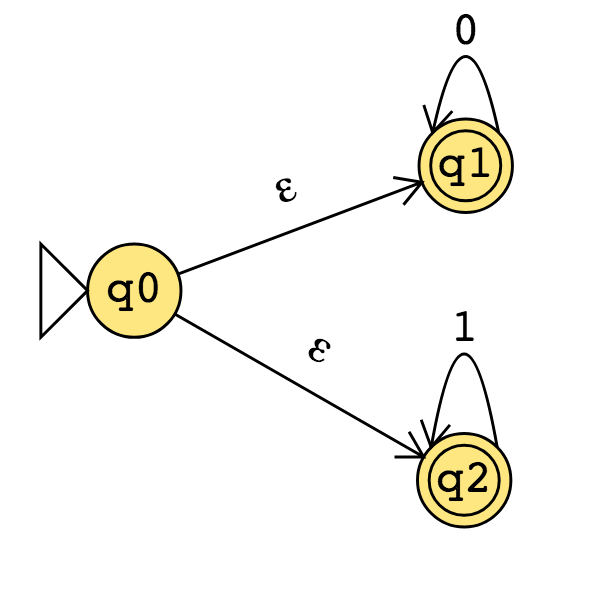
\includegraphics[width=1.8in]{../../resources/machines/Lect6NFA2.png}

\vspace{50pt}

Prune this diagram to get an 
equivalent DFA 
with only the ``macro-states" reachable from the start state.

\vspace{150pt}

Suppose $A$ is a language over an alphabet $\Sigma$.
{\bf Claim:} if there is a regular expression $R$ such that $L(R) = A$, then there is a NFA, let's call it $N$, such that 
$L(N) = A$.

{\bf Structural induction}: Regular expression is built from basis regular expressions using inductive steps
(union, concatenation, Kleene star symbols). Use constructions to mirror these in NFAs.


{\bf Application}: A state diagram for a NFA over $\{a,b\}$ that recognizes $L(a^* (ab)^*)$:

\vfill

\newpage

Suppose $A$ is a language over an alphabet $\Sigma$.
{\bf Claim:} if there is a DFA $M$ such that $L(M) = A$, then there is a regular expression, let's call it $R$, such that 
$L(R) = A$.

{\bf Proof idea}: Trace all possible paths from start state to accept state.  Express labels of these paths
as regular expressions, and union them all.

\begin{enumerate}
\item Add new start state with $\varepsilon$ arrow to old start state.
\item Add new accept state with $\varepsilon$ arrow from old accept states.  Make old accept states
non-accept.
\item Remove one (of the old) states at a time: modify regular expressions on arrows that went through removed
state to restore language recognized by machine.
\end{enumerate}

{\bf Application}: Find a regular expression describing the language recognized by the DFA with 
state diagram

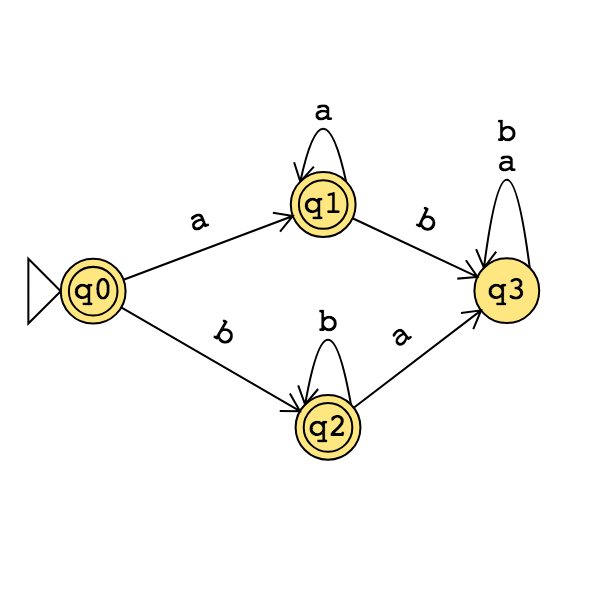
\includegraphics[width=2.5in]{../../resources/machines/Lect6NFA3.png}

\vfill


\newpage

{\bf Conclusion}: For each language $L$,
\begin{center}
    {\bf There is a DFA that recognizes $L$ \qquad $\exists M ~(M \textrm{ is a DFA and } L(M) = A)$}\\
    {\bf if and only if}\\
    {\bf There is a NFA that recognizes $L$  \qquad $\exists N ~(N \textrm{ is a NFA and } L(N) = A)$}\\
    {\bf if and only if}\\
    {\bf There is a regular expression that describes $L$ $\exists R ~(R \textrm{ is a regular expression and } L(R) = A)$}\\
\end{center}

A language is called {\bf regular} when any (hence all) of the above three conditions are met.

\subsection*{Review: Week 3 Wednesday}

Please complete the review quiz questions on \href{http://gradescope.com}{Gradescope} about 
translating between DFA, NFA, and regular expressions.


{\bf Pre class reading for next time}: Introduction to Section 1.4 (page 77)



\newpage
\subsection*{Friday}

%! app: regular-languages
%! outcome: Classify language, Find example languages, Pumping Lemma


{\bf Theorem}: For an alphabet $\Sigma$, For each language $L$ over $\Sigma$, 
\begin{center}
$L$ is recognized by some DFA \\
iff\\
$L$ is recognized by some NFA\\
iff\\
$L$ is described by some regular expression
\end{center}
If (any, hence all) these conditions apply, $L$ is called {\bf regular}.



{\bf Prove or Disprove}: There is some alphabet $\Sigma$ for which there is 
some language recognized by an NFA but not by any DFA.

\vspace{30pt}

{\bf Prove or Disprove}: There is some alphabet $\Sigma$ for which there is 
some finite language not described by any regular expression over $\Sigma$.

\vspace{30pt}


{\bf Prove or Disprove}: If a language is recognized by an NFA 
then the complement of this language is not recognized by any DFA.

\vspace{30pt}


\newpage
\begin{center}
\begin{tabular}{c|c}
Set & Cardinality \\
\hline
& \\
$\{0,1\}$ & \\
& \\
$\{0,1\}^*$ & \\
& \\
$\mathcal{P}( \{0,1\})$ & \\
& \\
The set of all languages over $\{0,1\}$ & \\
& \\
The set of all regular expressions over $\{0,1\}$ & \\
& \\
The set of all regular languages over $\{0,1\}$ & \\
& \\
\end{tabular}
\end{center}



\vfill

\newpage

{\bf Pumping Lemma} (Sipser Theorem 1.70): If $A$ is a regular language, then there
is a number $p$ (a {\it pumping length}) where, if $s$ is any string in $A$ of length at least $p$, 
then $s$ may be divided into three pieces, $s = xyz$ such that
\vspace{-10pt}
\begin{itemize}
\item $|y| > 0$
\item for each $i \geq 0$, $xy^i z \in A$
\item $|xy| \leq p$.
\end{itemize}


{\bf True or False}: A pumping length for $A = \{ 0,1 \}^*$ is $p = 5$.

\vspace{100pt}

{\bf True or False}: A pumping length for $A = \{1, 01, 001, 0001, 00001 \}$ is $p = 4$.

\vspace{100pt}

{\bf True or False}: A pumping length for $A = \{0^j 1 \mid  j \geq 0 \}$ is $p = 3$.


\vspace{100pt}

{\bf True or False}: For any language $A$, if $p$  is a  pumping length for $A$ and $p' > p$,  then 
$p'$ is also a pumping length for $A$.


\subsection*{Review: Week 3 Friday}


Please complete the review quiz questions on \href{http://gradescope.com}{Gradescope} about 
the class of regular languages.

{\bf Pre class reading for next time}: Example 1.75, Example 1.77
\newpage

\section*{Monday}

%! app: regular-languages
%! outcome: Classify language, Find example languages, Pumping Lemma

Recap so far: In DFA, the only memory available is in the states. Automata can only
``remember'' finitely far in the past and finitely much information, because
they can have only finitely many states. If a computation path of a DFA visits 
the same state more than once, the machine can't tell the difference between 
the first time and future times it visits this state. Thus, if 
a DFA accepts one long string, then it must accept (infinitely) many 
similar strings.

{\bf Definition}  A positive integer $p$ is a {\bf pumping length} of a language $L$ over $\Sigma$ means
that, for each string $s  \in  \Sigma^*$, if  $|s| \geq p$ and $s \in L$, then there are strings $x,y,z$
such that 
\[
s = xyz
\]
and  
\[
|y| > 0,  \qquad \qquad 
\text{ for each $i \geq 0$, $xy^i z \in L$}, \qquad \text{and}
\qquad  \qquad
|xy| \leq p.
\]

{\bf Negation}: A positive integer  $p$  is {\bf not a pumping length} of a language  $L$ over  $\Sigma$  iff
\[
\exists s \left(~  |s| \geq  p \wedge s \in L \wedge \forall x \forall y \forall z  \left( ~\left( s = xyz \wedge 
|y| > 0 \wedge |xy| \leq p~ \right) \to \exists i  (  i \geq 0  \wedge xy^iz  \notin L ) \right) ~\right) 
\]
{\it Informally: }


Restating {\bf Pumping Lemma}: If $L$ is a regular language, then it  has
a pumping length.


{\bf Contrapositive}: If $L$ has no pumping length, then  it is nonregular.

\vfill

{\Large The Pumping Lemma {\it cannot} be used to prove that a language {\it is} regular.} 

{\Large The Pumping Lemma {\bf can} be used to prove that a language {\it is not} regular.}

{\it Extra practice}: Exercise 1.49 in the book.


\vfill

{\bf Proof strategy}: To prove that a language $L$ is {\bf not} regular, 
\begin{itemize}
    \item Consider an arbitrary positive integer $p$
    \item Prove that $p$ is not a pumping length for $L$
    \item Conclude that $L$ does not have {\it any} pumping length, and therefore it is not regular.
\end{itemize}

\newpage
{\bf Example}: $\Sigma  =  \{0,1\}$, $L = \{ 0^n 1^n \mid n  \geq 0\}$.

Fix $p$ an arbitrary positive integer. List strings that are in $L$ and have length  greater than or equal  to $p$:

\vspace{20pt}

Pick $s = $


Suppose $s = xyz$ with  $|xy|  \leq  p$ and $|y| > 0$.
\begin{center}
\begin{tabular}{|c|}
\hline
 \\
\hspace{4in} \\
\hline
\end{tabular}
\end{center}

Then when $i = \hspace{1in}$, $xy^i z  = \hspace{1in}$

\newpage

{\bf Example}: $\Sigma  =  \{0,1\}$, $L = \{w w^{\mathcal{R}} \mid w \in \{0,1\}^*\}$.

Fix $p$ an arbitrary positive integer. List strings that are in $L$ and have length  greater than or equal  to $p$:

\vspace{10pt}

Pick $s = $

Suppose $s = xyz$ with  $|xy|  \leq  p$ and $|y| > 0$.
\begin{center}
\begin{tabular}{|c|}
\hline
 \\
\hspace{4in} \\
\hline
\end{tabular}
\end{center}
Then when $i = \hspace{1in}$, $xy^i z  = \hspace{1in}$


\vspace{30pt} 

{\bf Example}: $\Sigma  =  \{0,1\}$, $L = \{0^j1^k  \mid j \geq k  \geq 0\}$.

Fix $p$ an arbitrary positive integer. List strings that are in $L$ and have length  greater than or equal  to $p$:

\vspace{10pt}

Pick $s = $


Suppose $s = xyz$ with  $|xy|  \leq  p$ and $|y| > 0$.
\begin{center}
\begin{tabular}{|c|}
\hline
 \\
\hspace{4in} \\
\hline
\end{tabular}
\end{center}
Then when $i = \hspace{1in}$, $xy^i z  = \hspace{1in}$



\vspace{30pt} 

{\bf Example}: $\Sigma  =  \{0,1\}$, $L = \{0^n1^t0^n  \mid m,n  \geq 0\}$.

Fix $p$ an arbitrary positive integer. List strings that are in $L$ and have length  greater than or equal  to $p$:

\vspace{10pt}

Pick $s = $


Suppose $s = xyz$ with  $|xy|  \leq  p$ and $|y| > 0$.
\begin{center}
\begin{tabular}{|c|}
\hline
 \\
\hspace{4in} \\
\hline
\end{tabular}
\end{center}
Then when $i = \hspace{1in}$, $xy^i z  = \hspace{1in}$

    
\subsection*{Review: Week 4 Monday}


Recall: Review quizzes based on class material are assigned each day. 
These quizzes will help you track and confirm your understanding of the concepts and examples 
we work in class. Quizzes can be submitted on Gradescope as many times (with no penalty) as 
you like until the quiz deadline: the three quizzes each week are all due on Friday (with no penalty 
late submission open until Sunday).

Please complete the review quiz questions on \href{http://gradescope.com}{Gradescope} about 
pumping lemma and nonregular sets.

{\bf Pre class reading for next time}: Page 112


\newpage
\subsection*{Wednesday}

%! app: regular-languages, context-free-languages
%! outcome: Formal definition of automata, Informal definition of automata, Nondeterminism, Classify language


\begin{center}
    \begin{tabular}{c|c| c| c}
    Language & $s \in L$ & $s \notin L$ & Is the language regular or nonregular?  \\
    \hline
     & \hspace{1in} & \hspace{1in}  &  \\
    $\{a^nb^n \mid 0  \leq n  \leq 5 \}$ & & & \\
     & & & \\
    $\{b^n a^n \mid  n  \geq 2\}$  & & & \\
     & & & \\
    $\{a^m b^n \mid  0 \leq m\leq n\}$  & & & \\
     & & & \\
    $\{a^m b^n \mid  m \geq n+3,  n \geq 0\}$  & & & \\
     & & & \\
    $\{b^m a^n \mid  m \geq 1, n \geq  3\}$  & & & \\
     & & & \\
    $\{ w  \in \{a,b\}^* \mid w = w^\mathcal{R} \}$ & & & \\
     & & & \\ 
    $\{ ww^\mathcal{R} \mid w\in \{a,b\}^* \}$ & & & \\
     & & & \\ 
    \end{tabular}
\end{center}
    
\newpage
Regular sets are not the end of the story
\begin{itemize}
    \item Many nice / simple / important sets are not regular
    \item Limitation of the finite-state automaton model: Can't "count", Can only remember finitely far into the past,
    Can't backtrack, Must make decisions in "real-time"
    \item We know actual computers are more powerful than this model...
\end{itemize}

The {\bf next} model of computation. Idea: allow some memory of unbounded size. How? 
\begin{itemize}
    \item To generalize regular expressions: {\bf context-free grammars}\\
    \item To generalize NFA: {\bf Pushdown automata}, which is like an NFA with access to a stack: 
    Number of states is fixed, number of entries in stack is unbounded. At each step
    (1) Transition to new state based on current state, letter read, and top letter of stack, then
    (2) (Possibly) push or pop a letter to (or from) top of stack. Accept a string iff
    there is some sequence of states and some sequence of stack contents 
    which helps the PDA processes the entire input string and ends in an accepting state.
\end{itemize}

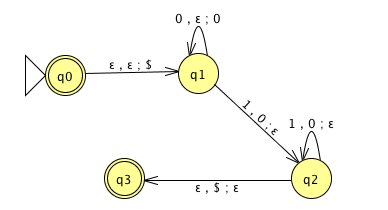
\includegraphics[width=4in]{../../resources/machines/Lect9PDA.png}
    
Trace the computation of this PDA on the input string $01$.

\vspace{80pt}  
    
Trace the computation of this PDA on the input string $011$.

\vspace{80pt}


\subsection*{Review: Week 4 Wednesday}

Please complete the review quiz questions on \href{http://gradescope.com}{Gradescope} about 
PDA definitions.

{\bf Pre class reading for next time}: Page 102



\newpage
\subsection*{Friday}

%! app: regular-languages, context-free-languages
%! outcome: Formal definition of automata, Informal definition of automata, Nondeterminism, Classify language, Find example languages

Consider the state diagram of a PDA with input alphabet 
$\Sigma$ and stack alphabet $\Gamma$.

\vspace{-0.2in}

\begin{center}
\begin{tabular}{|c|c|}
\hline
Label & means \\
\hline
$a, b \to c$ when $a \in \Sigma$, $b\in \Gamma$, $c \in \Gamma$ 
& \hspace{3in} \\
& \\
&\\
\hline
$a, \varepsilon \to c$ when $a \in \Sigma$, $c \in \Gamma$ 
& \hspace{3in} \\
& \\
&\\
\hline
$a, b \to \varepsilon$ when $a \in \Sigma$, $b\in \Gamma$
& \hspace{3in} \\
& \\
&\\
\hline
$a, \varepsilon \to \varepsilon$ when $a \in \Sigma$
& \hspace{3in} \\
& \\
&\\
\hline
\end{tabular}
\end{center}

\vspace{-0.2in}

How does the meaning change if $a$ is replaced by $\varepsilon$?


For the PDA state diagrams below, $\Sigma = \{0,1\}$.


\vspace{-0.2in}


\begin{center}
\begin{tabular}{c c}
Mathematical description of language & State diagram of PDA recognizing language\\
\hline
& 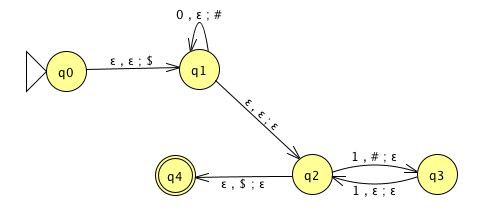
\includegraphics[width=3.5in]{../../resources/machines/Lect10PDA1.png}\\
\hline
& 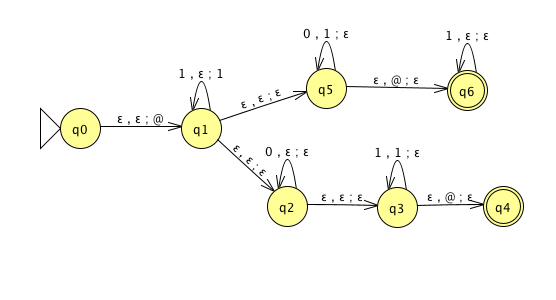
\includegraphics[width=3.5in]{../../resources/machines/Lect10PDA2.png}\\
\hline
& \\
$\{ 0^i 1^j 0^k \mid i,j,k \geq 0 \}$ & \\
\end{tabular}
\end{center}

\newpage

Assume $a \in \Sigma$ and $L$ is a language over $\Sigma$.  Recall that 
\[
aL = \{ aw \mid w \in L \}
\]
If $M = (Q, \Sigma, \Gamma, \delta, q_0, F)$ is a PDA with $L(M) = L$, 
a PDA $M_1$ that recognizes $aL$ is
\[
M_1 = ( \hspace{1in} , \Sigma, \Gamma, \delta_1, \hspace{0.5in}, \hspace{0.5in})
\]
with

\vspace{180pt}



\newpage
\subsection*{Review: Week 4 Friday}


Please complete the review quiz questions on \href{http://gradescope.com}{Gradescope} about 
PDA construction.


\newpage

\section*{Monday}

%! app: context-free languages
%! outcome: Classify language, Find example languages, context-free grammars

To fully specify a PDA we could give its $6$-tuple formal definition or we could give its input 
alphabet, stack alphabet, and state diagram.
An informal description of a PDA is a step-by-step description of how its computations 
would process input strings; the reader should be able to reconstruct the state diagram or formal 
definition precisely from such a descripton. The informal description of a PDA can refer to some 
common modules or subroutines that are computable by PDAs:
\begin{itemize}
  \item PDAs can ``test for emptyness of stack'' without providing details. 
  {\it How?} We can always push a special end-of-stack symbol, $\$$, at the start, before processing
  any input, and then use this symbol as a flag.
  \item PDAs can ``test for end of input'' without providing details.
  {\it How?} We can transform a PDA to one where accepting states are only those reachable 
  when there are no more input symbols.
\end{itemize}


  \newpage
  
  Design a CFG to generate the  language $\{abba\}$
  
  \begin{align*}
  & ( \{ S, T, V, W\}, \{a,b\}, \{ S \to aT, T \to bV, V \to bW, W \to a\}, S)\\
  & \\ 
  & \\ 
  & \\ 
  & ( \{ Q \}, \{a,b\}, \{Q \to abba\}, Q) \\
  & \\ 
  & \\ 
  & \\
  & ( \{ X,Y \}, \{a,b\}, \{X \to aYa, Y \to bb\}, X) 
  & \\ 
  & \\ 
  \end{align*} 


  Design a CFG to generate the  language $\{a^n b^n \mid  n  \geq  0\}$
  
  \vspace{150pt}
  
  {\it Sample derivation:} 
  
  \vspace{30pt}
  
  
  Design a CFG to generate the  language $\{a^i b^j \mid j \geq i  \geq 0\}$
  
  \vspace{150pt}
  
  {\it Sample derivation:} 
  
  \vspace{30pt}

    
\newpage
\subsection*{Review: Week 5 Monday}


Recall: Review quizzes based on class material are assigned each day. 
These quizzes will help you track and confirm your understanding of the concepts and examples 
we work in class. Quizzes can be submitted on Gradescope as many times (with no penalty) as 
you like until the quiz deadline: the three quizzes each week are all due on Friday (with no penalty 
late submission open until Sunday).

Please complete the review quiz questions on \href{http://gradescope.com}{Gradescope} about 
context-free grammars

{\bf Pre class reading for next time}: Figure 3.1 (Pages 165-167)

\newpage
\subsection*{Wednesday}

%! app: context-free languages
%! outcome: Classify language, Find example languages, context-free grammars, Formal definition of automata, Informal definition of automata

    
A set $X$ is said to be {\bf closed} under an operation $OP$ if, for any elements in $X$, applying 
$OP$ to them gives an element in $X$.  


\begin{center}
\begin{tabular}{|c|l|}
\hline
True/False & Closure claim \\
\hline
True &  The set of integers is closed under multiplication. \\
& $\forall x \forall y \left( ~(x \in \mathbb{Z} \wedge y \in \mathbb{Z})\to xy \in \mathbb{Z}~\right)$ \\
\hline
True & For each set $A$, the power set of $A$ is closed under intersection. \\
& $\forall A_1 \forall A_2 \left( ~(A_1 \in \mathcal{P}(A) \wedge A_2 \in \mathcal{P}(A) \in \mathbb{Z}) \to A_1 \cap A_2 \in \mathcal{P}(A)~\right)$ \\
\hline
  & The class of regular languages over $\Sigma$ is closed under complementation. \\
  & \\
 \hline
  & The class of regular languages over $\Sigma$ is closed under union. \\
  & \\
 \hline
  & The class of regular languages over $\Sigma$ is closed under intersection. \\
  & \\
  \hline
  & The class of regular languages over $\Sigma$ is closed under concatenation. \\
  & \\
 \hline
  & The class of regular languages over $\Sigma$ is closed under Kleene star. \\
  & \\
\hline
    & The class of context-free languages over $\Sigma$ is closed under complementation. \\
  & \\
\hline
    & The class of context-free languages over $\Sigma$ is closed under union. \\
  & \\
\hline
    & The class of context-free languages over $\Sigma$ is closed under intersection. \\
  & \\
\hline
    & The class of context-free languages over $\Sigma$ is closed under concatenation. \\
  & \\
\hline
    & The class of context-free languages over $\Sigma$ is closed under Kleene star. \\
  & \\
\hline
\end{tabular}
\end{center}

\vfill

Assume  $\Sigma  = \{0,1, \#\}$
\begin{center}
\begin{tabular}{|cc|}
\hline
&\\
$\Sigma^*$  & Regular ~~/~~ nonregular and context-free ~~/~~not context-free\\

$\{0^i\# 1^j \mid i \geq  0, j  \geq 0\}$  & Regular ~~/~~ nonregular and context-free ~~/~~not context-free\\

$\{0^i1^j\# 1^j0^i \mid i \geq  0, j  \geq 0\}$  & Regular ~~/~~ nonregular and context-free ~~/~~not context-free\\

$\{0^i1^j\# 0^i 1^j \mid i \geq  0, j  \geq 0\}$  & Regular ~~/~~ nonregular and context-free ~~/~~not context-free\\
&\\
\hline
\end{tabular}
\end{center}

\newpage
{\bf Turing machines}: unlimited read + write memory, unlimited time (computation can proceed
without ``consuming'' input and can re-read symbols of input)
\begin{itemize}
\item Division betweeen program (CPU, state diagram) and data
\item Unbounded memory gives theoretical limit to what modern computation 
(including PCs, supercomputers, quantum computers) can achieve
\item State diagram formulation is simple enough to reason about (and diagonalize against) while
expressive enough to capture modern computation
\end{itemize}

For Turing machine $M= (Q, \Sigma, \Gamma, \delta, q_0, q_{accept}, q_{reject})$ 
the {\bf computation} of $M$ on a string $w$ over $\Sigma$  is:

\vspace{-20pt}

\begin{itemize}
\setlength{\itemsep}{0pt}
\item Read/write head starts at leftmost position on tape. 
\item Input string is written on $|w|$-many leftmost cells of tape, 
rest of  the tape cells have  the blank symbol. {\bf Tape alphabet} 
is $\Gamma$ with $\textvisiblespace\in \Gamma$ and $\Sigma \subseteq \Gamma$.
The blank symbol $\textvisiblespace \notin \Sigma$.
\item Given current state of machine and current symbol being read at the tape head, 
the machine transitions to next state, writes a symbol to the current position  of the 
tape  head (overwriting existing symbol), and moves the tape head L or R (if possible). 
Formally, {\bf transition function}  is 
\[
  \delta: Q\times \Gamma \to Q \times \Gamma \times \{L, R\}
\]
\item Computation ends if and when machine enters either the accept or the reject state.
This is called {\bf halting}.
Note: $q_{accept} \neq q_{reject}$.
\end{itemize}

The {\bf language recognized by the  Turing machine} $M$,  is  
\[
  \{ w \in \Sigma^* \mid \textrm{computation of $M$ on $w$ halts after entering the accept state}\} = \{ w \in \Sigma^* \mid w \textrm{ is accepted by } M\}
\]

\newpage
An example Turing machine: $\Sigma = \phantom{\hspace{1in}}, \Gamma = \phantom{\hspace{1in}} $
\[
  \delta ( ( q0, 0)  ) =  
\]

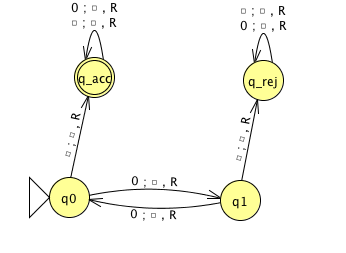
\includegraphics[width=2.5in]{../../resources/machines/Lect13TM1.png}

Formal definition: 


Sample computation: 

\begin{tabular}{|c|c|c|c|c|c|c|}
\hline
\multicolumn{1}{|c}{$q0\downarrow$} &  \multicolumn{6}{c|}{\phantom{A}}\\
\hline
$0$ & $0$  & $0$ & $\textvisiblespace $& $\textvisiblespace $& $\textvisiblespace $&  $\textvisiblespace $\\
\hline
\multicolumn{7}{|c|}{\phantom{A}}\\
\hline
\phantom{AA} & \phantom{AA}& \phantom{AA}& \phantom{AA}& \phantom{AA}& \phantom{AA}& \phantom{AA} \\
\hline
\multicolumn{7}{|c|}{\phantom{A}}\\
\hline
\phantom{AA} & \phantom{AA}& \phantom{AA}& \phantom{AA}& \phantom{AA}& \phantom{AA}& \phantom{AA} \\
\hline
\multicolumn{7}{|c|}{\phantom{A}}\\
\hline
\phantom{AA} & \phantom{AA}& \phantom{AA}& \phantom{AA}& \phantom{AA}& \phantom{AA}& \phantom{AA} \\
\hline
\multicolumn{7}{|c|}{\phantom{A}}\\
\hline
\phantom{AA} & \phantom{AA}& \phantom{AA}& \phantom{AA}& \phantom{AA}& \phantom{AA}& \phantom{AA} \\
\hline
\end{tabular}

\vfill

The language recognized by this machine is \ldots

{\it Extra practice:}

 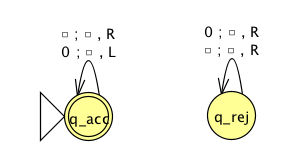
\includegraphics[width=2in]{../../resources/machines/Lect13TM2.png} 


 Formal definition: 


 Sample computation: 
 


\newpage
\subsection*{Review: Week 5 Wednesday}

Please complete the review quiz questions on \href{http://gradescope.com}{Gradescope} about 
context-free languages and Turing machines.


\newpage
\subsection*{Friday: Midterm exam}

{\bf The midterm exam policies are below}

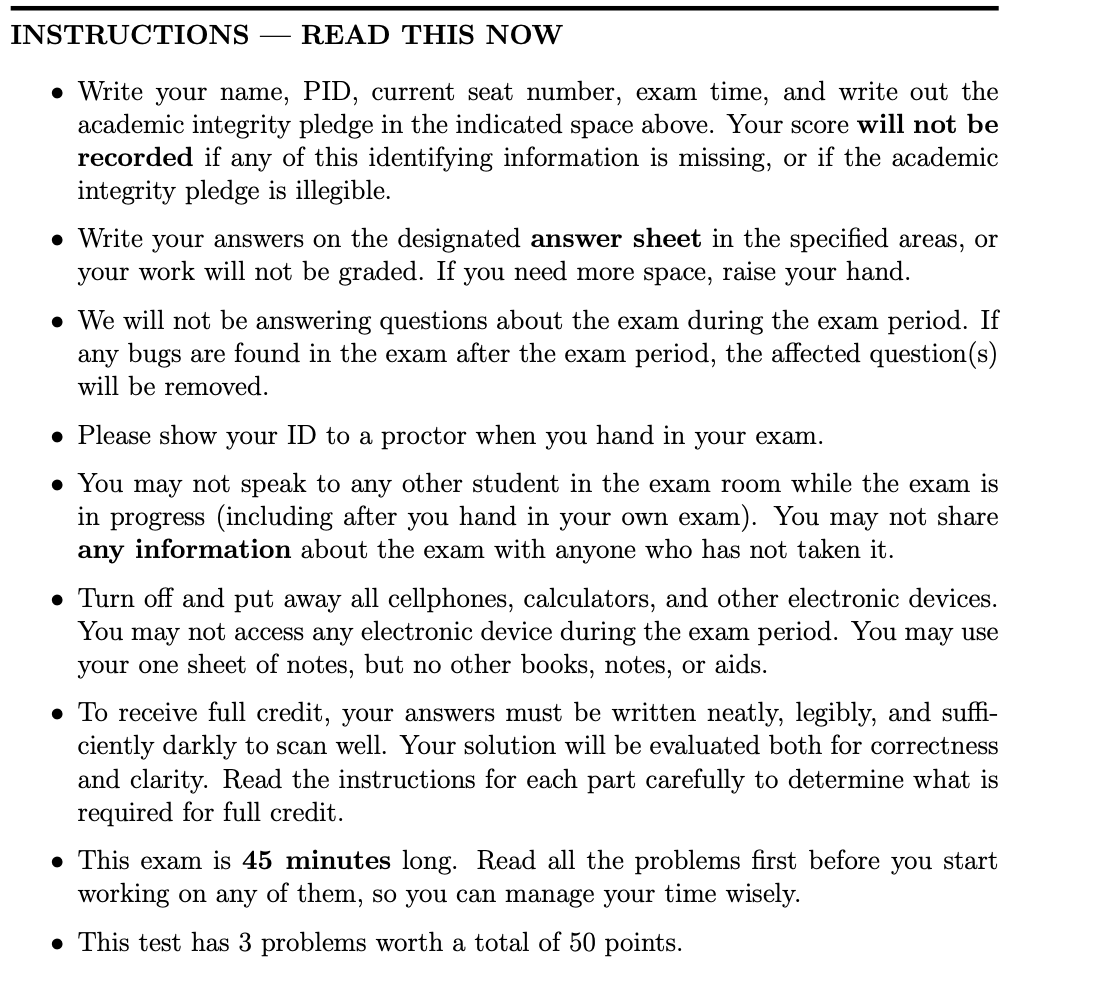
\includegraphics[width=\linewidth]{../../files/midterm-instructions.png}
\newpage

\section*{Monday}

%! app: decidable languages, undecidable languages
%! outcome: Formal definition of automata, Informal definition of automata, Classify language, Find example languages
    
For Turing machine $M= (Q, \Sigma, \Gamma, \delta, q_0, q_{accept}, q_{reject})$ 
the {\bf computation} of $M$ on a string $w$ over $\Sigma$  is:

\vspace{-20pt}

\begin{itemize}
\setlength{\itemsep}{0pt}
\item Read/write head starts at leftmost position on tape. 
\item Input string is written on $|w|$-many leftmost cells of tape, 
rest of  the tape cells have  the blank symbol. {\bf Tape alphabet} 
is $\Gamma$ with $\textvisiblespace\in \Gamma$ and $\Sigma \subseteq \Gamma$.
The blank symbol $\textvisiblespace \notin \Sigma$.
\item Given current state of machine and current symbol being read at the tape head, 
the machine transitions to next state, writes a symbol to the current position  of the 
tape  head (overwriting existing symbol), and moves the tape head L or R (if possible). 
Formally, {\bf transition function}  is 
\[
  \delta: Q\times \Gamma \to Q \times \Gamma \times \{L, R\}
\]
\item Computation ends if and when machine enters either the accept or the reject state.
This is called {\bf halting}.
Note: $q_{accept} \neq q_{reject}$.
\end{itemize}

The {\bf language recognized by the  Turing machine} $M$,  is  
\[
  \{ w \in \Sigma^* \mid \textrm{computation of $M$ on $w$ halts after entering the accept state}\} = \{ w \in \Sigma^* \mid w \textrm{ is accepted by } M\}
\]
  
To define a Turing machine, we could give a 
\begin{itemize}
\item {\bf Formal definition}, namely the $7$-tuple of parameters including set of states, 
input alphabet, tape alphabet, transition function, start state, accept state, and reject state; or,
\item {\bf Implementation-level definition}: English prose that describes the Turing machine head 
movements relative to contents of tape, and conditions for accepting / rejecting based on those contents.
\end{itemize}

Conventions for drawing state diagrams of Turing machines: (1) omit the reject state from the diagram (unless 
it's the  start state), (2) any missing transitions in the state diagram have value $(q_{reject}, ~\textvisiblespace~ , R)$.


\newpage
{\it Sipser Figure  3.10}

\begin{multicols}{2}
\vspace{-20pt}
\begin{center}
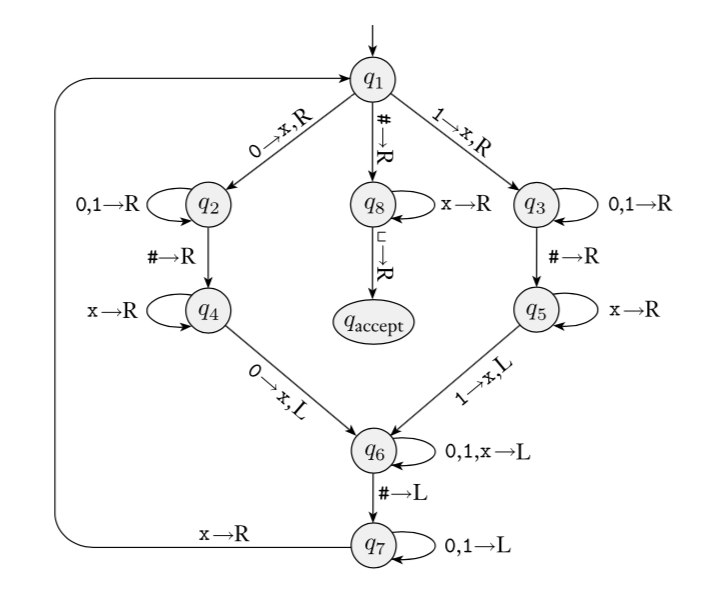
\includegraphics[width=4in]{../../resources/machines/Lect13TM3.png}
\end{center}

Implementation level description of this machine:
\begin{quote}
Zig-zag across tape to corresponding positions on either side of $\#$ to check whether the 
characters in these positions agree. If they do not, or if there is no $\#$, reject. If they 
do, cross them off.

Once all symbols to the left of the $\#$ are crossed off, check for any un-crossed-off symbols 
to the right of $\#$; if there are any, reject; if there aren't, accept.
\end{quote}

\columnbreak

Computation on  input  string  $01\#01$

\begin{tabular}{|c|c|c|c|c|c|c|}
\hline
\multicolumn{1}{|c}{$q_1 \downarrow$} &  \multicolumn{6}{c|}{\phantom{A}}\\
\hline
$0$ & $1$  & $\#$  & $0$ & $1$ & $\textvisiblespace $& $\textvisiblespace $\\
\hline
  \multicolumn{7}{|c|}{\phantom{A}}\\
  \hline
  \phantom{AA} & \phantom{AA}& \phantom{AA}& \phantom{AA}& \phantom{AA}& \phantom{AA}& \phantom{AA} \\
  \hline
  \multicolumn{7}{|c|}{\phantom{A}}\\
  \hline
  \phantom{AA} & \phantom{AA}& \phantom{AA}& \phantom{AA}& \phantom{AA}& \phantom{AA}& \phantom{AA} \\
  \hline
  \multicolumn{7}{|c|}{\phantom{A}}\\
  \hline
  \phantom{AA} & \phantom{AA}& \phantom{AA}& \phantom{AA}& \phantom{AA}& \phantom{AA}& \phantom{AA} \\
  \hline
  \multicolumn{7}{|c|}{\phantom{A}}\\
  \hline
  \phantom{AA} & \phantom{AA}& \phantom{AA}& \phantom{AA}& \phantom{AA}& \phantom{AA}& \phantom{AA} \\
  \hline
  \multicolumn{7}{|c|}{\phantom{A}}\\
  \hline
  \phantom{AA} & \phantom{AA}& \phantom{AA}& \phantom{AA}& \phantom{AA}& \phantom{AA}& \phantom{AA} \\
  \hline
  \multicolumn{7}{|c|}{\phantom{A}}\\
  \hline
  \phantom{AA} & \phantom{AA}& \phantom{AA}& \phantom{AA}& \phantom{AA}& \phantom{AA}& \phantom{AA} \\
  \hline
  \multicolumn{7}{|c|}{\phantom{A}}\\
  \hline
  \phantom{AA} & \phantom{AA}& \phantom{AA}& \phantom{AA}& \phantom{AA}& \phantom{AA}& \phantom{AA} \\
  \hline
  \multicolumn{7}{|c|}{\phantom{A}}\\
  \hline
  \phantom{AA} & \phantom{AA}& \phantom{AA}& \phantom{AA}& \phantom{AA}& \phantom{AA}& \phantom{AA} \\
  \hline
  \multicolumn{7}{|c|}{\phantom{A}}\\
  \hline
  \phantom{AA} & \phantom{AA}& \phantom{AA}& \phantom{AA}& \phantom{AA}& \phantom{AA}& \phantom{AA} \\
  \hline
  \multicolumn{7}{|c|}{\phantom{A}}\\
  \hline
  \phantom{AA} & \phantom{AA}& \phantom{AA}& \phantom{AA}& \phantom{AA}& \phantom{AA}& \phantom{AA} \\
  \hline
  \multicolumn{7}{|c|}{\phantom{A}}\\
  \hline
  \phantom{AA} & \phantom{AA}& \phantom{AA}& \phantom{AA}& \phantom{AA}& \phantom{AA}& \phantom{AA} \\
  \hline
  \multicolumn{7}{|c|}{\phantom{A}}\\
  \hline
  \phantom{AA} & \phantom{AA}& \phantom{AA}& \phantom{AA}& \phantom{AA}& \phantom{AA}& \phantom{AA} \\
  \hline
  \multicolumn{7}{|c|}{\phantom{A}}\\
  \hline
  \phantom{AA} & \phantom{AA}& \phantom{AA}& \phantom{AA}& \phantom{AA}& \phantom{AA}& \phantom{AA} \\
  \hline
  \multicolumn{7}{|c|}{\phantom{A}}\\
  \hline
  \phantom{AA} & \phantom{AA}& \phantom{AA}& \phantom{AA}& \phantom{AA}& \phantom{AA}& \phantom{AA} \\
  \hline
  \multicolumn{7}{|c|}{\phantom{A}}\\
  \hline
  \phantom{AA} & \phantom{AA}& \phantom{AA}& \phantom{AA}& \phantom{AA}& \phantom{AA}& \phantom{AA} \\
  \hline
  \multicolumn{7}{|c|}{\phantom{A}}\\
  \hline
  \phantom{AA} & \phantom{AA}& \phantom{AA}& \phantom{AA}& \phantom{AA}& \phantom{AA}& \phantom{AA} \\
  \hline
  \multicolumn{7}{|c|}{\phantom{A}}\\
  \hline
  \phantom{AA} & \phantom{AA}& \phantom{AA}& \phantom{AA}& \phantom{AA}& \phantom{AA}& \phantom{AA} \\
  \hline
  \multicolumn{7}{|c|}{\phantom{A}}\\
  \hline
  \phantom{AA} & \phantom{AA}& \phantom{AA}& \phantom{AA}& \phantom{AA}& \phantom{AA}& \phantom{AA} \\
  \hline
  \end{tabular}
\end{multicols}

The language recognized by this machine is
\[
  \{ w \# w \mid w \in \{0,1\}^* \}
\]

\newpage

  A language $L$ is {\bf recognized by} a Turing machine $M$ means

  \vspace{20pt}

  A Turing  machine  $M$ {\bf  recognizes} a language $L$ if means

  \vspace{20pt}
  
  A Turing machine $M$ is a {\bf decider}  means

  \vspace{20pt}
  
  A language  $L$ is {\bf decided by} a Turing  machine  $M$  means

  \vspace{20pt}
  
  A  Turing machine $M$ {\bf decides} a language $L$ means

  \vspace{20pt}
  
  
  Fix $\Sigma = \{0,1\}$, $\Gamma = \{ 0, 1, \textvisiblespace\}$ for the Turing machines with  the following state diagrams:
  
  \vspace{-35pt}
  
  
  \begin{center}
  \begin{tabular}{|c|c|}
  \hline
  \hspace{0.8in}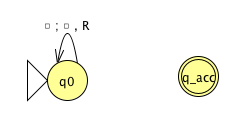
\includegraphics[width=2in]{../../resources/machines/Lect14TM1.png} \phantom{\hspace{0.8in}}&\hspace{0.8in} 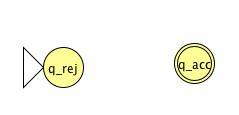
\includegraphics[width=2in]{../../resources/machines/Lect14TM2.png} \phantom{\hspace{0.8in}}\\
  Implementation  level description:  \phantom{\hspace{1in}} &Implementation  level description:  \phantom{\hspace{1in}} \\
  &\\
  &\\
  &\\
  Example of string accepted: \phantom{\hspace{1.5in}}& Example of string accepted: \phantom{\hspace{1.5in}}\\
  Example of string rejected: \phantom{\hspace{1.5in}}& Example of string  rejected: \phantom{\hspace{1.5in}}\\
  &\\
  Decider? Yes~~~/ ~~~No
  &Decider? Yes~~~/ ~~~No\\
  & \\
  \hline
  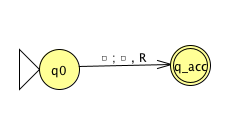
\includegraphics[width=2in]{../../resources/machines/Lect14TM3.png} & 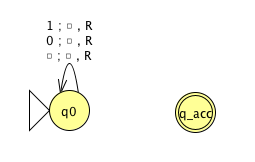
\includegraphics[width=2in]{../../resources/machines/Lect14TM4.png} \\
  Implementation  level description:  \phantom{\hspace{1in}} &Implementation  level description:  \phantom{\hspace{1in}} \\
  &\\
  &\\
  &\\
  Example of string accepted: \phantom{\hspace{1.5in}}& Example of string accepted: \phantom{\hspace{1.5in}}\\
  Example of string rejected: \phantom{\hspace{1.5in}}& Example of string  rejected: \phantom{\hspace{1.5in}}\\
  &\\
  Decider? Yes~~~/ ~~~No
  &Decider? Yes~~~/ ~~~No\\
  & \\
  
  \hline
  \end{tabular}
  \end{center}
    
\newpage
\subsection*{Review: Week 6 Monday}


Recall: Review quizzes based on class material are assigned each day. 
These quizzes will help you track and confirm your understanding of the concepts and examples 
we work in class. Quizzes can be submitted on Gradescope as many times (with no penalty) as 
you like until the quiz deadline: the three quizzes each week are all due on Friday (with no penalty 
late submission open until Sunday).

Please complete the review quiz questions on \href{http://gradescope.com}{Gradescope} about 
formal and implementation-level descriptions of Turing machines.

{\bf Pre class reading for next time}: pages 176-177 on variants of Turing machines


\newpage
\subsection*{Wednesday}

%! app: Decidable Languages, Undecidable Languages
%! outcome: Formal definition of automata, Informal definition of automata, Classify language, Find example languages
    

  
  Fix $\Sigma = \{0,1\}$, $\Gamma = \{ 0, 1, \textvisiblespace\}$ for the Turing machines with  the following state diagrams:
  
  \begin{center}
  \begin{tabular}{|c|c|}
  \hline
  \hspace{0.8in}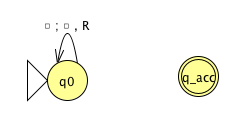
\includegraphics[width=2in]{../../resources/machines/Lect14TM1.png} \phantom{\hspace{0.8in}}&\hspace{0.8in} 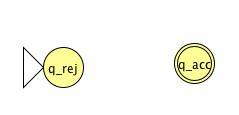
\includegraphics[width=2in]{../../resources/machines/Lect14TM2.png} \phantom{\hspace{0.8in}}\\
  Implementation  level description:  \phantom{\hspace{1in}} &Implementation  level description:  \phantom{\hspace{1in}} \\
  &\\
  &\\
  &\\
  Example of string accepted: \phantom{\hspace{1.5in}}& Example of string accepted: \phantom{\hspace{1.5in}}\\
  Example of string rejected: \phantom{\hspace{1.5in}}& Example of string  rejected: \phantom{\hspace{1.5in}}\\
  & \\
  \hline
  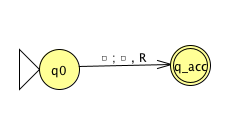
\includegraphics[width=2in]{../../resources/machines/Lect14TM3.png} & 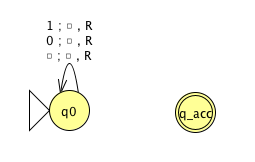
\includegraphics[width=2in]{../../resources/machines/Lect14TM4.png} \\
  Implementation  level description:  \phantom{\hspace{1in}} &Implementation  level description:  \phantom{\hspace{1in}} \\
  &\\
  &\\
  &\\
  Example of string accepted: \phantom{\hspace{1.5in}}& Example of string accepted: \phantom{\hspace{1.5in}}\\
  Example of string rejected: \phantom{\hspace{1.5in}}& Example of string  rejected: \phantom{\hspace{1.5in}}\\
  & \\
  
  \hline
  \end{tabular}
  \end{center}

Two models of computation are called {\bf equally expressive} when 
every language recognizable with the first model is recognizable with the second, and vice versa.

True / False: NFAs and PDAs are equally expressive.

True / False: Regular expressions and CFGs are equally expressive.


To say a language is {\bf Turing-recognizable} means that there is some Turing machine that recognizes it.

\begin{center}
{\large \it  Some examples of models that are {\bf equally expressive} with deterministic Turing machines: }
\end{center}

\newpage
\fbox{ {\bf May-stay}  machines }
The May-stay machine model is the same as the usual Turing machine model,  except that
on each transition, the tape head may move L, move R, or Stay. 

Formally: $(Q, \Sigma, \Gamma, \delta, q_0, q_{accept}, q_{reject})$ where 
\[
  \delta: Q \times \Gamma \to Q \times \Gamma \times \{L, R, S\}
\]

{\bf Claim}: Turing machines and May-stay machines are equally expressive. {\it To prove \ldots}

To translate a standard TM to a may-stay machine: 

\vspace{100pt}




To translate one  of the  may-stay machines to standard TM:
any time TM would Stay, move right  then  left.


Formally: suppose $M_S =  (Q, \Sigma, \Gamma, \delta, q_0, q_{acc}, q_{rej})$
has $\delta: Q \times \Gamma \to Q \times \Gamma \times \{L, R, S\}$. Define
the Turing-machine
\[
  M_{new} =  (\phantom{\hspace{2.5in}})
\]

\vfill


\phantom{$M_{new}$ construction here \vspace{400pt}}
\vfill

\newpage

\fbox{ {\bf Multitape Turing machine}} A multitape Turing macihne with $k$ tapes
can be formally representated as 
$(Q, \Sigma,  \Gamma, \delta, q_0, q_{acc}, q_{rej})$ 
where $Q$ is the finite set of  states,
$\Sigma$ is the  input alphabet with  $\textvisiblespace \notin \Sigma$,
$\Gamma$  is the  tape alphabet with $\Sigma \subsetneq \Gamma$ ,
$\delta: Q\times \Gamma^k\to Q \times \Gamma^k \times \{L,R\}^k$ 
(where $k$ is  the number of  states)


If $M$ is a standard  TM, it is a $1$-tape machine.


To translate a $k$-tape machine  to  a standard TM:
Use a  new symbol to separate the contents of each tape
and keep track of location of  head with  special version of each
tape symbol. {\tiny Sipser Theorem 3.13} 

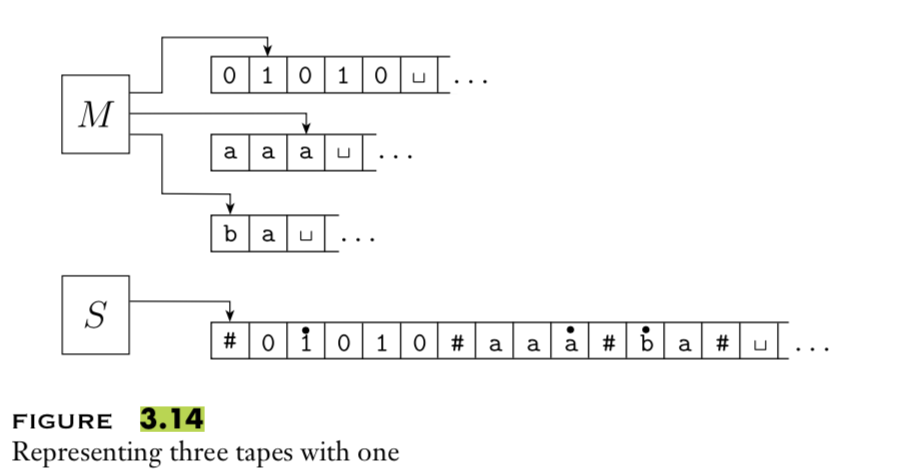
\includegraphics[width=2.5in]{../../resources/images/Figure314.png}

\vfill

{\it Extra practice:} \fbox{ {\bf  Wikipedia Turing machine} }
Define a machine $(Q, \Gamma, b, \Sigma,  q_0, F, \delta)$
where $Q$ is the finite set  of  states
$\Gamma$  is the tape alphabet,
$b \in \Gamma$ is the blank symbol, 
$\Sigma \subsetneq \Gamma$ is the  input alphabet, 
$q_0 \in  Q$ is the start state, 
$F \subseteq Q$ is the set of accept states, 
$\delta: (Q \setminus F)  \times  \Gamma \not\to Q \times  \Gamma  \times \{L, R\}$
 is a partial transition function
If computation enters a state  in $F$, it  accepts 
If computation enters a configuration where
 $\delta$ is not defined, it  rejects . {\tiny Hopcroft and  Ullman, cited by  Wikipedia} 

\vfill

\newpage
\fbox{ {\bf Enumerators} } Enumerators give a different
model of computation where a language is {\bf produced, one string at a time},
rather than recognized by accepting (or not) individual strings.

Each enumerator machine has finite state control, unlimited work tape, and a printer. The computation proceeds
according to transition function; at any point machine may ``send'' a string to the printer.
\[
E  = (Q, \Sigma, \Gamma, \delta, q_0, q_{print})  
\]
$Q$ is the finite set of states, $\Sigma$ is  the output alphabet, $\Gamma$ is the 
tape alphabet ($\Sigma  \subsetneq\Gamma, 
\textvisiblespace \in \Gamma \setminus \Sigma$), 
\[
\delta:  Q  \times  \Gamma \times \Gamma \to  Q \times  \Gamma \times  \Gamma \times \{L, R\} \times  \{L, R\}
\]
where in state $q$, when the working tape is scanning character $x$ and the printer tape is scanning character $y$,
$\delta( (q,x,y) ) = (q', x', y', d_w, d_p)$ means transition to control state $q'$, write $x'$ on 
the working tape, write $y'$ on the printer tape, move in direction $d_w$ on the working tape, and move in direction 
$d_p$ on the printer tape. The computation starts in $q_0$ and each time the computation enters $q_{print}$
the string from the leftmost edge of the printer tape to the first blank cell is considered to be printed.

The language  {\bf  enumerated} by  $E$, $L(E)$, is $\{ w \in \Sigma^* \mid \text{$E$ eventually, at finite  time, 
prints $w$} \}$.


\begin{center}
\begin{tabular}{cc}
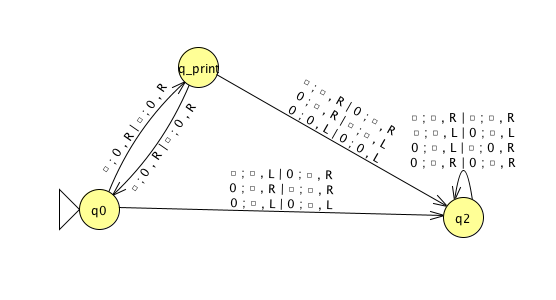
\includegraphics[width=3.5in]{../../resources/machines/Lec15enumerator.png}  & 
\begin{tabular}{|c|c|c|c|c|c|c|}
\hline
\multicolumn{1}{|c}{$q0$} &  \multicolumn{6}{c|}{\phantom{A}}\\
\hline
$\textvisiblespace ~*$& $\textvisiblespace$  & $\textvisiblespace$ & $\textvisiblespace$& $\textvisiblespace$& $\textvisiblespace$&  $\textvisiblespace$\\
\hline
$\textvisiblespace  ~*$& $\textvisiblespace$  & $\textvisiblespace$ & $\textvisiblespace$& $\textvisiblespace$& $\textvisiblespace$&  $\textvisiblespace$\\
\hline\hline
\multicolumn{7}{|c|}{\phantom{A}}\\
\hline
\phantom{AA} & \phantom{AA}& \phantom{AA}& \phantom{AA}& \phantom{AA}& \phantom{AA}& \phantom{AA} \\
\hline
\phantom{AA} & \phantom{AA}& \phantom{AA}& \phantom{AA}& \phantom{AA}& \phantom{AA}& \phantom{AA} \\
\hline
\hline
\multicolumn{7}{|c|}{\phantom{A}}\\
\hline
\phantom{AA} & \phantom{AA}& \phantom{AA}& \phantom{AA}& \phantom{AA}& \phantom{AA}& \phantom{AA} \\
\hline
\phantom{AA} & \phantom{AA}& \phantom{AA}& \phantom{AA}& \phantom{AA}& \phantom{AA}& \phantom{AA} \\
\hline
\hline
\multicolumn{7}{|c|}{\phantom{A}}\\
\hline
\phantom{AA} & \phantom{AA}& \phantom{AA}& \phantom{AA}& \phantom{AA}& \phantom{AA}& \phantom{AA} \\
\hline
\phantom{AA} & \phantom{AA}& \phantom{AA}& \phantom{AA}& \phantom{AA}& \phantom{AA}& \phantom{AA} \\
\hline
\hline
\multicolumn{7}{|c|}{\phantom{A}}\\
\hline
\phantom{AA} & \phantom{AA}& \phantom{AA}& \phantom{AA}& \phantom{AA}& \phantom{AA}& \phantom{AA} \\
\hline
\phantom{AA} & \phantom{AA}& \phantom{AA}& \phantom{AA}& \phantom{AA}& \phantom{AA}& \phantom{AA} \\
\hline
\end{tabular}
\end{tabular}
\end{center}


\newpage

{\bf Theorem 3.21} A language is Turing-recognizable iff some enumerator enumerates it.

{\bf Proof}:

Assume $L$ is enumerated by some enumerator, $E$, so $L = L(E)$.
We'll use $E$ in a subroutine
within a high-level description of a new Turing machine that we will build to recognize $L$.

{\bf Goal}: build Turing machine $M_E$ with $L(M_E) = L(E)$.

Define $M_E$ as follows: $M_E = $ ``On input $w$,
\begin{enumerate}
\item Run $E$. For each string $x$ printed by $E$.
\item \qquad Check if $x = w$. If so, accept (and halt); otherwise, continue."
\end{enumerate}


\vfill 



Assume $L$ is Turing-recognizable and there 
is a Turing  machine  $M$ with  $L = L(M)$. We'll use $M$ in a subroutine
within a high-level description of an enumerator that we will build to enumerate $L$.

{\bf Goal}: build enumerator $E_M$ with $L(E_M) = L(M)$.

{\bf Idea}: check each string in turn to see if it is in $L$.

{\it How?} Run computation of $M$ on each string.  {\it But}: need to be careful 
about computations that don't halt.

{\it Recall} String order for $\Sigma = \{0,1\}$: $s_1 = \varepsilon$, $s_2 = 0$, $s_3 = 1$, $s_4 = 00$, $s_5 = 01$, $s_6  = 10$, 
$s_7  =  11$, $s_8 = 000$, \ldots

Define $E_M$ as follows: $E_{M} = $ `` {\it ignore any input.} Repeat the following for $i=1, 2, 3, \ldots$
\begin{enumerate}
  \item Run the computations of $M$ on $s_1$, $s_2$, \ldots, $s_i$ for (at most) $i$ steps each
  \item For each of these $i$ computations that accept during the (at most) $i$ steps, print
  out the accepted string."
\end{enumerate}


\newpage
\subsection*{Review: Week 6 Wednesday}

Please complete the review quiz questions on \href{http://gradescope.com}{Gradescope} about 
variants of Turing machines.

{\bf Pre class reading for next time}: Theorem 3.16 on page 178 (nondeterministism)



\newpage
\subsection*{Friday}

%! app: decidable languages, undecidable languages
%! outcome: Formal definition of automata, Informal definition of automata, Classify language, Find example languages, Nondeterminism, Church-Turing


To define a Turing machine, we could give a 
\begin{itemize}
\item {\bf Formal definition}: the $7$-tuple of parameters including set of states, 
input alphabet, tape alphabet, transition function, start state, accept state, and reject state; or,
\item {\bf Implementation-level definition}: English prose that describes the Turing machine head 
movements relative to contents of tape, and conditions for accepting / rejecting based on those contents.
\item {\bf High-level description}: description of algorithm (precise sequence of instructions), 
without implementation details of machine. As part of this description, can ``call" and run 
another TM as a subroutine.
\end{itemize}


{\bf Theorem 3.21} A language is Turing-recognizable iff some enumerator enumerates it.

{\bf Proof}:

Assume $L$ is enumerated by some enumerator, $E$, so $L = L(E)$.
We'll use $E$ in a subroutine
within a high-level description of a new Turing machine that we will build to recognize $L$.

{\bf Goal}: build Turing machine $M_E$ with $L(M_E) = L(E)$.

Define $M_E$ as follows: $M_E = $ ``On input $w$,
\begin{enumerate}
\item Run $E$. For each string $x$ printed by $E$.
\item \qquad Check if $x = w$. If so, accept (and halt); otherwise, continue."
\end{enumerate}


\vfill 



Assume $L$ is Turing-recognizable and there 
is a Turing  machine  $M$ with  $L = L(M)$. We'll use $M$ in a subroutine
within a high-level description of an enumerator that we will build to enumerate $L$.

{\bf Goal}: build enumerator $E_M$ with $L(E_M) = L(M)$.

{\bf Idea}: check each string in turn to see if it is in $L$.

{\it How?} Run computation of $M$ on each string.  {\it But}: need to be careful 
about computations that don't halt.

{\it Recall} String order for $\Sigma = \{0,1\}$: $s_1 = \varepsilon$, $s_2 = 0$, $s_3 = 1$, $s_4 = 00$, $s_5 = 01$, $s_6  = 10$, 
$s_7  =  11$, $s_8 = 000$, \ldots

Define $E_M$ as follows: $E_{M} = $ `` {\it ignore any input.} Repeat the following for $i=1, 2, 3, \ldots$
\begin{enumerate}
  \item Run the computations of $M$ on $s_1$, $s_2$, \ldots, $s_i$ for (at most) $i$ steps each
  \item For each of these $i$ computations that accept during the (at most) $i$ steps, print
  out the accepted string."
\end{enumerate}

\newpage

{\bf Nondeterministic Turing machine}

At any point in the computation, the nondeterministic machine may proceed according to 
several possibilities: $(Q, \Sigma, \Gamma, \delta, q_0, q_{acc}, q_{rej})$ where 
\[
\delta: Q \times \Gamma \to \mathcal{P}(Q \times \Gamma \times \{L, R\})  
\]
The computation of a nondeterministic Turing machine is a tree with branching
when the next step of the computation has multiple possibilities. A nondeterministic
Turing machine accepts a string exactly when some branch of the computation tree 
enters the accept state.

Given a nondeterministic machine, we can use a $3$-tape Turing machine to 
simulate it by doing a breadth-first search of computation tree: one tape 
is ``read-only'' input tape, one tape simulates the tape of the nondeterministic
computation, and one tape tracks nondeterministic branching. {\tiny Sipser page 178} 

\vfill
Two models of computation are called {\bf equally expressive} when 
every language recognizable with the first model is recognizable with the second, and vice versa.

{\bf  Church-Turing Thesis} (Sipser p. 183): The informal notion of algorithm is formalized completely  and correctly by the 
formal definition of a  Turing machine. In other words: all reasonably expressive models of 
computation are equally expressive with the standard Turing machine.

\vfill

\newpage

{\bf Claim}: If two languages  (over a fixed alphabet  $\Sigma$) are Turing-recognizable, then  their union  is  as well.

{\bf Proof using Turing machines}:

\vfill

{\bf Proof using nondeterministic Turing machines}: 

\vfill  

{\bf  Proof using enumerators}:

\vfill



\newpage
\subsection*{Review: Week 6 Friday}


Please complete the review quiz questions on \href{http://gradescope.com}{Gradescope} about 
descriptions of Turing machines.

{\bf Pre class reading for next time}: Page 184-185 Terminology for describing Turing machines


\newpage

\section*{Monday}

%! app: Decidable Languages, Undecidable Languages
%! outcome: Classify language, Find example languages, Define decision problem, Classify decision problem
    

\begin{center}
    \begin{tabular}{|l|l|l|l|}
    \hline
    & Suppose $M$ is  a TM & Suppose $D$ is  a TM & Suppose $E$ is  an
    enumerator  \\
    &that  recognizes $L$  &that  decides $L$  &that enumerates $L$ \\
    \hline
    If string $w$ is in  $L$ then  \ldots  &&& \\
    &&&\\
    &&&\\
    If string $w$ is not in  $L$ then  \ldots  && &\\
    &&&\\
    &&&\\
    \hline
    \end{tabular}
\end{center}


A language $L$ is {\bf recognized by} a Turing machine $M$ means

\vspace{15pt}

A Turing  machine  $M$ {\bf  recognizes} a language $L$ if means

\vspace{15pt}

A Turing machine $M$ is a {\bf decider}  means

\vspace{15pt}

A language  $L$ is {\bf decided by} a Turing  machine  $M$  means

\vspace{15pt}

A  Turing machine $M$ {\bf decides} a language $L$ means

\vspace{15pt}


{\it From Friday's review quiz: }
Which of the following sentences make sense? Which of those are true?

A language is a decider if it always halts.

\vfill

The union of two deciders is a decider.

\vfill

A language is decidable if and only if it is recognizable.

\vfill

There is a Turing machine that isn't decidable.

\vfill

There is a recognizable language that isn't decided by any Turing machine.

\vfill

\newpage


{\bf Claim}: If two languages  (over a fixed alphabet  $\Sigma$) are Turing-recognizable, then  their union  is  as well.

{\bf Proof using Turing machines}:

\vfill

{\bf Proof using nondeterministic Turing machines}: 

\vfill  

{\bf  Proof using enumerators}:

\vfill

\newpage


The first line of a {\bf high-level description} of a Turing machine specifies the input to the machine, which must be a string.
This string may be the encoding of some object or  list of  objects.  

{\bf Notation:} $\langle O \rangle$ is the string that encodes the object $O$.
$\langle O_1, \ldots, O_n \rangle$ is the string that encodes the list of objects $O_1, \ldots, O_n$.

{\bf Assumption}: There are Turing  machines that can be called as subroutines
to decode the string representations of common objects and  interact with these objects as intended
(data structures).
  
For example, since there are algorithms to answer each of the following questions,
by Church-Turing thesis, there is a Turing machine that accepts exactly those strings for which the 
answer to the question is ``yes''
\begin{itemize}
    \item Does a string over $\{0,1\}$ have even length?

    \vfill

    \item Does a string over $\{0,1\}$ encode a string of ASCII characters?\footnote{An introduction to ASCII 
    is available on the w3 tutorial \href{https://www.w3schools.com/charsets/ref_html_ascii.asp}{here}.}

    \vfill

    \item Does a DFA have a specific number of states?

    \vfill

    \item Do two NFAs have any state names in common?

    \vfill

    \item Do two CFGs have the same start variable?

    \vfill

  \end{itemize}

A {\bf computational problem} is decidable iff language encoding its positive problem instances
is decidable.

The computational problem ``Does a specific DFA accept a given string?'' is encoded by the language
\begin{align*}
  &\{ \textrm{representations of DFAs $M$ and strings $w$ such that $w \in L(M)$}\}  \\
  =& \{ \langle M, w \rangle \mid M \textrm{ is a DFA}, w \textrm{ is a string}, w \in L(M) \}
\end{align*}

The computational problem ``Is the language generated by a CFG empty?'' is encoded by the language
\begin{align*}
  &\{ \textrm{representations of CFGs $G$  such that $L(G) = \emptyset$}\}  \\
  =& \{ \langle G \rangle \mid G \textrm{ is a CFG},  L(G) = \emptyset \}
\end{align*}



The computational problem ``Is the given Turing machine a decider?'' is encoded by the language
\begin{align*}
  &\{ \textrm{representations of TMs $M$  such that $M$ halts on every input}\}  \\
  =& \{ \langle M \rangle \mid M \textrm{ is a TM and for each string } w, \textrm{$M$ halts on $w$} \}
\end{align*}


{\it Note: writing down the language encoding a computational problem is only the first step in 
determining if it's recognizable, decidable, or \ldots }

    
\newpage
\subsection*{Review: Week 7 Monday}


Recall: Review quizzes based on class material are assigned each day. 
These quizzes will help you track and confirm your understanding of the concepts and examples 
we work in class. Quizzes can be submitted on Gradescope as many times (with no penalty) as 
you like until the quiz deadline: the three quizzes each week are all due on Friday (with no penalty 
late submission open until Sunday).

Please complete the review quiz questions on \href{http://gradescope.com}{Gradescope} about 
computational problems.

{\bf Pre class reading for next time}: Decidable problems concerning regular languages, Sipser pages 194-196.


\newpage
\subsection*{Wednesday}

%! app: decidable languages, undecidable languages
%! outcome: Classify language, Find example languages, Define decision problem, Classify decision problem
    
Deciding a computational problem means building / defining a Turing 
machine that recognizes the language encoding the computational problem, and that 
is a decider.

\begin{center}
  \begin{tabular}{|lcl|}
  \hline
  \multicolumn{3}{|l|}{{\bf  Acceptance problem} } \\
  for \ldots  & $A_{\ldots}$ & $\{ \langle B,w \rangle \mid  \text{$B$ is a \ldots that accepts input 
  string $w$}\}$ \\
  \hline
  \multicolumn{3}{|l|}{{\bf Language emptiness  testing} } \\
   for \ldots & $E_{\ldots}$ & $\{ \langle A \rangle \mid  \text{$A$ is a \ldots and  $L(A) = \emptyset$\}}$ \\
  \hline
  \multicolumn{3}{|l|}{{\bf Language equality testing} } \\
   for \ldots & $EQ_{\ldots}$ & $\{ \langle A, B \rangle \mid  \text{$A$ and $B$ are \ldots and  $L(A) =L(B)$\}}$\\
  \hline
  Sipser Section 4.1 &&\\
  \hline
  \end{tabular}
  \end{center}
  
  \begin{quote}
  $M_1 = $ ``On input $\langle M,w\rangle$, where $M$ is a DFA and $w$ is a string:
  \begin{enumerate}
  \setcounter{enumi}{-1}
  \item Type check encoding to check input is correct type.
  \item Simulate $M$ on input $w$ (by keeping track of states in $M$, transition function of $M$, etc.) 
  \item If the simulations ends in an accept state of $M$, accept. If it ends in a non-accept state of $M$, reject. "
  \end{enumerate}
  \end{quote}
  

What is $L(M_1)$? 

\vfill

Is $L(M_1)$ a decider?

\vfill

  
  \begin{quote}
  $M_2 =  $``On  input  $\langle M, w \rangle$ where $M$ is a  DFA and  $w$ is  a string, 
  \begin{enumerate}
  \item Run $M$ on  input  $w$.
  \item If $M$  accepts, accept; if $M$ rejects, reject."
  \end{enumerate}
  \end{quote}
  

  What is $L(M_2)$? 

  \vfill
  
  Is $L(M_2)$ a decider?
  
  \vfill
  
    
\newpage
  $A_{REX} = $

  $A_{NFA} = $


  True / False: $A_{REX} = A_{NFA} = A_{DFA}$

  True / False: $A_{REX} \cap A_{NFA} = \emptyset$, $A_{REX} \cap A_{DFA} = \emptyset$, $A_{DFA} \cap A_{NFA} = \emptyset$

  
  A Turing machine that  decides $A_{NFA}$ is: 
  
  \vfill
  
  A Turing machine that  decides $A_{REX}$ is: 
  
  \vfill
  \newpage
  
  \begin{quote}
  $M_3 =  $``On  input  $\langle M\rangle$ where $M$ is a  DFA,
  \begin{enumerate}
  \item For integer  $i = 1, 2, \ldots$
  \item \qquad Let  $s_i$ be the  $i$th string over  the alphabet of  $M$ (ordered in  string order).
  \item \qquad Run $M$ on  input  $s_i$.
  \item \qquad If $M$  accepts,  $\underline{\phantom{FILL  IN BLANK}}$.  If $M$  rejects, increment $i$ and keep going."
  \end{enumerate}
  \end{quote}
  

Choose the correct option to help fill in the blank so that $M_3$ recognizes $E_{DFA}$
\begin{itemize}
\item[A.] accepts
\item[B.] rejects
\item[C.] loop for ever
\item[D.] We can't fill in the blank in any way to make this work
\item[E.] None of the above
\end{itemize}

  
  \begin{quote}
  $M_4 =  $ `` On  input $\langle M \rangle$ where $M$ is  a  DFA,
  \begin{enumerate}
  \item Mark the start  state  of $M$.
  \item Repeat until no  new states get marked:
  \item \qquad Loop over the states of $M$. 
  \item \qquad Mark any unmarked  state  that  has an incoming  edge  from a marked state.
  \item If  no  accept state of $A$ is  marked, $\underline{\phantom{FILL  IN BLANK}}$;  otherwise, 
  $\underline{\phantom{FILL  IN BLANK}}$".
  \end{enumerate}
  \end{quote}
  
  
  
To build a Turing machine that decides $EQ_{DFA}$, notice that 
\[
L_1 = L_2 \qquad\textrm{iff}\qquad (~(L_1 \cap \overline{L_2}) \cup (L_2 \cap \overline L_1)~) = \emptyset  
\]
{\it There are no elements that are in one set and not the other}


$M_{EQDFA} = $ 


  \vfill
  
  \newpage
  {\bf Summary}:  We can use the decision procedures (Turing machines) of decidable problems
  as subroutines in other algorithms. For example, we have subroutines for deciding each of 
  $A_{DFA}$, $E_{DFA}$, $EQ_{DFA}$.  We can also use algorithms for known constructions
  as subroutines in other algorithms. For example, we have subroutines for: counting the number 
  of states in a state diagram, counting the number of characters in an alphabet, converting DFA
  to a DFA recognizing the complement of the original language or a DFA recognizing the 
  Kleene star of the original language, constructing a DFA or NFA from two DFA or NFA so that 
  we have a machine recognizing the language of the union (or intersection, concatenation)
  of the languages of the original machines; converting regular expressions to equivalent DFA; 
  converting DFA to equivalent regular expressions, etc.



\subsection*{Review: Week 7 Wednesday}

Please complete the review quiz questions on \href{http://gradescope.com}{Gradescope} about 
decidable computational problems.

{\bf Pre class reading for next time}: An undecidable language, Sipser pages 207-209.



\newpage
\subsection*{Friday}

%! app: decidable languages, undecidable languages
%! outcome: Classify language, Find example languages, Define decision problem, Classify decision problem
    

A {\bf Turing-recognizable} language is a set of strings that 
is the language recognized by some Turing machine. We also 
say that such languages are recognizable.

A {\bf Turing-decidable} language is a set of strings that 
is the language recognized by some decider. We also 
say that such languages are decidable.

An {\bf unrecognizable} language is a language that is not Turing-recognizable.

An {\bf undecidable} language is a language that is not Turing-decidable.


{\bf  True} or {\bf False}: Any  undecidable language  is  also  unrecognizable.


{\bf  True} or {\bf False}: Any  unrecognizable language  is  also  undecidable.


To prove that a computational problem is {\bf decidable}, we find/ build a Turing 
machine that recognizes the language encoding the computational problem, and that 
is a decider.


How do we prove a specific problem is {\bf not decidable}?

How would we even find such a computational problem?


{\it Counting arguments for the existence of an undecidable language:}
\begin{itemize}
    \item The set of all Turing machines is countably infinite.
    \item Each Turing-recognizable language is associated with a Turing machine
    in a one-to-one relationship, so there can be no more Turing-recognizable
    languages than there are Turing machines. 
    \item Since there are infinitely many Turing-recognizable languages
    (think of the singleton sets), there are countably infinitely 
    many Turing-recognizable languages.
    \item Such the set of Turing-decidable languages is an infinite subset 
    of the set of Turing-recognizable languages, the set of 
    Turing-decidable languages is also countably infinite.
\end{itemize}

Since there are uncountably many languages (because $\mathcal{P}{\Sigma^*}$
is uncountable), there are uncountably many unrecognizable languages
and there are uncountably many undecidable languages.

\vfill

{\bf What's a specific example of a language that is unrecognizable or undecidable?}

{\bf Key idea}: self-referential disagreement.

\newpage
\begin{center}
\begin{tabular}{|lcl|}
\hline
\multicolumn{3}{|l|}{{\bf  Acceptance problem} } \\
for Turing  machines  & $A_{TM}$ & $\{ \langle M,w \rangle \mid  \text{$M$ is a Turing machine that accepts input 
string $w$}\}$ \\
\hline
\multicolumn{3}{|l|}{{\bf Language emptiness  testing} } \\
 for Turing machines & $E_{TM}$ & $\{ \langle M \rangle \mid  \text{$M$ is a Turing machine and  $L(M) = \emptyset$\}}$ \\
\hline
\multicolumn{3}{|l|}{{\bf Language equality testing} } \\
 for Turing machines& $EQ_{TM}$ & $\{ \langle  M_1, M_2 \rangle \mid  \text{$M_1$ and $M_2$ are Turing machines and  
 $L(M_1) =L(M_2)$\}}$\\
\hline
Sipser Section 4.1 &&\\
\hline
\end{tabular}
\end{center}

\begin{multicols}{3}
$M_1$ 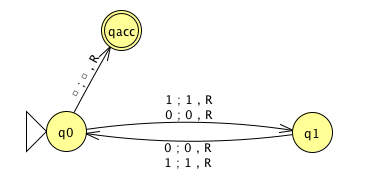
\includegraphics[width=2in]{../../resources/machines/Week8WarmupTM1.png} 

\columnbreak

$M_2$ 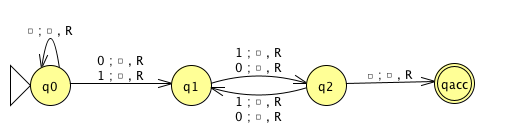
\includegraphics[width=2in]{../../resources/machines/Week8WarmupTM2.png}

\columnbreak

$M_3$ 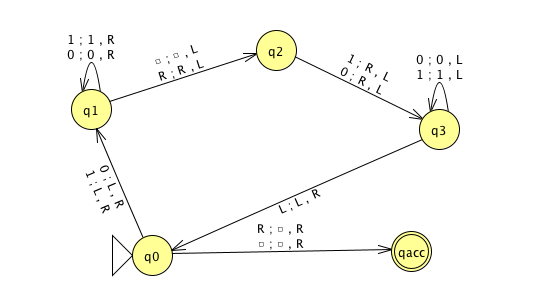
\includegraphics[width=2in]{../../resources/machines/Week8WarmupTM3.png}
\end{multicols}

Example strings in $A_{TM}$

\vfill

Example strings in  $E_{TM}$

\vfill

Example strings in  $EQ_{TM}$

\vfill

\newpage

{\bf  Theorem}: $A_{TM}$  is  Turing-recognizable.


{\bf  Strategy}:  To prove this theorem, we need  to  define  a Turing  machine  $R_{ATM}$ such that 
$L(R_{ATM}) = A_{TM}$.


Define $R_{ATM} =  $ ``

\vspace{150pt}


Proof of correctness: 


\vfill
\vfill

We will show that $A_{TM}$ is undecidable.

\newpage
\subsection*{Review: Week 7 Friday}


Please complete the review quiz questions on \href{http://gradescope.com}{Gradescope} about 
undecidability and unrecognizability.

\newpage
\end{document}